%to have line numbers
%\RequirePackage{lineno}
\documentclass[10pt, letterpaper]{article}      
\usepackage[margin=.1cm,font=small,labelfont=bf]{caption}[2007/03/09]
%\usepackage{endnotes}
%\let\footnote=\endnote
\usepackage{setspace}
\usepackage{longtable}                        
\usepackage{anysize}                          
\usepackage{natbib}                           
%\bibpunct{(}{)}{,}{a}{,}{,}                   
\bibpunct{(}{)}{,}{a}{}{,}                   
\usepackage{amsmath}
\usepackage[% draft,
pdftex]{graphicx} %draft is a way to exclude figures                
\usepackage{epstopdf}
\usepackage{hyperref}                             % For creating hyperlinks in cross references


% \usepackage[margins]{trackchanges}

% \note[editor]{The note}
% \annote[editor]{Text to annotate}{The note}
%    \add[editor]{Text to add}
% \remove[editor]{Text to remove}
% \change[editor]{Text to remove}{Text to add}

%TODO make it more standard before submission: \marginsize{2cm}{2cm}{1cm}{1cm}
\marginsize{1cm}{1cm}{.5cm}{.5cm}%{left}{right}{top}{bottom}   
					          % Helps LaTeX put figures where YOU want
 \renewcommand{\topfraction}{1}	                  % 90% of page top can be a float
 \renewcommand{\bottomfraction}{1}	          % 90% of page bottom can be a float
 \renewcommand{\textfraction}{0.0}	          % only 10% of page must to be text

 \usepackage{float}                               %latex will not complain to include float after float

\usepackage[table]{xcolor}                        %for table shading
\definecolor{gray90}{gray}{0.90}
\definecolor{orange}{RGB}{255,128,0}

\renewcommand\arraystretch{.9}                    %for spacing of arrays like tabular

%-------------------- my commands -----------------------------------------
\newenvironment{ig}[1]{
\begin{center}
 %\includegraphics[height=5.0in]{#1} 
 \includegraphics[height=3.3in]{#1} 
\end{center}}

 \newcommand{\cc}[1]{
\hspace{-.13in}$\bullet$\marginpar{\begin{spacing}{.6}\begin{footnotesize}\color{blue}{#1}\end{footnotesize}\end{spacing}}
\hspace{-.13in} }

%-------------------- END my commands -----------------------------------------



%-------------------- extra options -----------------------------------------

%%%%%%%%%%%%%
% footnotes %
%%%%%%%%%%%%%

%\long\def\symbolfootnote[#1]#2{\begingroup% %these can be used to make footnote  nonnumeric asterick, dagger etc
%\def\thefootnote{\fnsymbol{footnote}}\footnote[#1]{#2}\endgroup}	%see: http://help-csli.stanford.edu/tex/latex-footnotes.shtml

%%%%%%%%%%%
% spacing %
%%%%%%%%%%%

% \abovecaptionskip: space above caption
% \belowcaptionskip: space below caption
%\oddsidemargin 0cm
%\evensidemargin 0cm

%%%%%%%%%
% style %
%%%%%%%%%

%\pagestyle{myheadings}         % Option to put page headers
                               % Needed \documentclass[a4paper,twoside]{article}
%\markboth{{\small\it Politics and Life Satisfaction }}
%{{\small\it Adam Okulicz-Kozaryn} }

%\headsep 1.5cm
% \pagestyle{empty}			% no page numbers
% \parindent  15.mm			% indent paragraph by this much
% \parskip     2.mm			% space between paragraphs
% \mathindent 20.mm			% indent math equations by this much

%%%%%%%%%%%%%%%%%%
% extra packages %
%%%%%%%%%%%%%%%%%%

\usepackage{datetime}


\usepackage[latin1]{inputenc}
\usepackage{tikz}
\usetikzlibrary{shapes,arrows,backgrounds}


%\usepackage{color}					% For creating coloured text and background
%\usepackage{float}
\usepackage{subfig}                                     % for combined figures

\renewcommand{\ss}[1]{{\colorbox{blue}{\bf \color{white}{#1}}}}
\newcommand{\ee}[1]{\endnote{\vspace{-.10in}\begin{spacing}{1.0}{\normalsize #1}\end{spacing}\vspace{.20in}}}
\newcommand{\emd}[1]{\ExecuteMetaData[/tmp/tex]{#1}} % grab numbers  from stata

%TODO before submitting comment this out to get 'regular fornt'
\usepackage{sectsty}
\allsectionsfont{\normalfont\sffamily}
\usepackage{sectsty}
\allsectionsfont{\normalfont\sffamily}
\renewcommand\familydefault{\sfdefault}

\usepackage[margins]{trackchanges}
\usepackage{rotating}
\usepackage{catchfilebetweentags}

\usepackage{abstract}
\renewcommand{\abstractname}{}    % clear the title
\renewcommand{\absnamepos}{empty} % originally center
%-------------------- END extra options -----------------------------------------
\date{{}\today}
\title{  
The effect of social transfers and social capital on subjetive wellbeing of
elderly\footnote{This study was funded by grant \# 2016/21/B/HS4/03058 from
  Polish National Science Foundation (Narodowe Centrum Nauki).}
}
\author{
% Adam Okulicz-Kozaryn\thanks{EMAIL: adam.okulicz.kozaryn@gmail.com
%   \hfill I thank XXX.  All mistakes are mine.} \\
% {\small Rutgers - Camden  and Vistula University}
% and Leszek Morawski\thanks{EMAIL: l.morawski@vistula.edu.pl}\\
% {\small Polish Academy of Sciences and Vistula University}
}

\begin{document}

%%\setpagewiselinenumbers
%\modulolinenumbers[1]
%\linenumbers

\bibliographystyle{/home/aok/papers/root/tex/ecta}
\maketitle
\vspace{-.4in}
\begin{center}

\end{center}


\begin{abstract}
\noindent We investigate the effect of social transfers (especially pension) and
social capital (especially volunteering) on subjective wellbeing (SWB) of elderly using the latest (wave 6) Survey of Health, Ageing and Retirement in Europe
(SHARE). We find that the effect of volunteering on SWB is not much smaller or
even about as large as that of pensions. In general, the most SWB stems from volunteering about
every week, but there is already a substantial effect even if one volunteers only
about every month. We also find that the poor and the miidle
class seem to benefit more from volunteering than the rich.
We argue that volunteering can help increase elderly's subjective wellbeing amidst tightening budgets.
\end{abstract}
\vspace{.15in} 
\noindent{\sc Subjective Wellbeing (SWB), Life Satisfaction, Happiness, Aging,
  Elderly, Volunteering, Social Capital, Survey of Health, Ageing and Retirement in Europe (SHARE) 
}
\vspace{.25in} 

\begin{spacing}{1.4} %TODO MAYBE before submission can make it like 2.0
\rowcolors{1}{white}{gray90}

%  instead \ExecuteMetaData[../out/tex]{ginipov} do \emd{ginipov}

% \begin{figure}[H]
%  \includegraphics[height=3in]{../out/gov_res_trust.pdf}\centering\label{gov_res_trust}
% \caption{woo}
% \end{figure}


Population aging will be the key issue in this century, amd perhaps even in 
the third
millennium  \citep{stolnitz1992demographic}. Specifically, there are growing
concerns about sustainability of pensions and health care \citep{jurges12}. 
The problem of aging is clear in many European countries, for instance in
Germany, Europe's most populous country, and there is clearly a need for social
science research to address aging as one of the most important challenges of our
times \citep{vaupel2006redistributing}. Likewise, there is a problem in
Poland, for instance, finances  of Polish Social Security (Zaklad Ubezpieczen
Spolecznych, ZUS) % and healthcare spending on elderly
do not seem sustainable. 
%
Amidst growing concerns about sustainability of pensions and health care, we
know surprisingly little about effects of various policies on the wellbeing of the elderly.% and what are the tradeoffs.
In present study % predicting SWB
we are especially interested in substitution between economic
capital (social transfers) v social capital (volunteering). %TODO use this terminology more;
                                %definietly at least one more guess at the end
%collective social policy and individual believes/values.
%  We will also control for a number of person-level characteristics.
%Our audience is broad--anybody interested in well-being and quality of life.

Volunteering has been advocated by the United Nations, American and European
governments as a way to engage people in their local communities and improve
social capital, with the potential for public health benefits such as improving
health and overall wellbeing 
\citep{jenkinson2013volunteering}. Promotion of volunteering could be an
alternative 
strategy to sustained social transfers in an effort to achieve a decent
wellbeing (for other strategies see \citet[][sec. 2.4.5]{ferring10}. 

There is a need for new knowledge: better understanding of the determinants of
SWB enables to evaluate and possibly reform present retirement
institutions, such as pension programs, as well
as potentially generate new institutions to meet the demands of rapidly
increasing retirement population. SWB can serve as a yardstick to evalate
substitution and net effect from each factor. In present study we will use SWB
to measure net effects of social transfers and social capital.

There is a growing recognition of well-being/quality of life
indicators \citep{aok_lsPol16}. Traditional
measures of development, such as income, production, or consumption are too
simplistic. They do not capture the overall progress of our civilization. For
instance, gross domestic product increases when there is traffic congestion, but
clearly that is not 
progress. But even increase in household income does not necessarily
 create progress if there is growing income inequality. 
Other important ingredients of overall development and progress such as
discretionary time, mental and physical health are not caputured by monetary measures. We will
capture overall progress by using SWB yardstick.

%We know very little about the effect of social policy on wellbeing.
There is an abundant literature about the effect of welfare on SWB as recently
reviewed in \citet{aokJap14}.{Political scientists tend to focus on welfare and institutions at country
level \citep{alvarez09,pacek08b,radcliff13,pacek08r,radcliff01,bok10}. A popular measure of welfare is so called ``commodification.'' On the societal level, \citet[p. 36]{esping90} argued that ``the market becomes to the worker a prison within which it is imperative to
behave as a commodity in order to survive.''
%  When workers feel like they are a commodity that leads to lower SWB \citep{easterlin09}.
% Additionally,  \citet{lane00} contended that  markets are indifferent
% to the fate of individuals so when there is not a safety net, people
% have lower SWB.  
Commodification mostly means lack of or inadequate pensions, sickness benefits,
and unemployment compensation \citep{scruggs06Ba}. Our contribution is to zoom
in at person level and focus on elderly.} % There is even more research about the effect of personal income on
% happiness \citep{dolan08al,veenhoven12,helliwell14b}. 
% In general, both income and welfare increase SWB, at least up to a point. 
%
% Yet, there is clearly a gap: welfare is studied at aggregate level, usually 
% country level, and despite voluminous research linking income with SWB, there
% are very few studies about welfare or social transfers at person level, and
%  all these studies overlook social capital, notably volunteering. 
% BELOW MAYBE A FOOTNOTE TO FLOW BETTER
 There are surprisingly different relationships between SWB and its predictors
 depending on the level of analysis \citep{ashkanasy11}, and implications from research findings can be
misguided when taken from only one level of analysis \citep{klein00}.

%
 % Research focusing on aging and happiness takes into account income, but either
 % overlooks social transfers or volunteering or both.
 We start with a general hypothesis about social
 transfers and social capital, which is multi-dimensional, and we focus  on volunteering:\\
\noindent$H_1:$ The more social transfers and social capital, especially in the
form of volunteering, the more happiness.\\

Studies focusing on elderly and their wellbeing, either miss social
transfers or volunteering (they do not examine them simultaneously), and they
often measure only specific domains of wellbeing, not overall wellbeing. We hypothesize some tradeoff or substitution between social transfers and
social capital:\\ 

\noindent$H_2:$ The more social capital, especially in the form of volunteering, the lower the need for social transfers to achieve happiness.\\ 


\section{Literature}

% focus on def of voluntering as among elderly
% Dictionary defines volunteering as
% definintion: voluntering: altruistic, etc
% \url{https://www.google.pl/search?q=volunteering+definition&rlz=1CATAAC_enUS742US743&oq=volunteering+definition&aqs=chrome..69i57j0l5.4820j0j7&sourceid=chrome&ie=UTF-8}
% The key of definition is altruism

Snyder and Omoto (2008, pp. 3-5) %from lm 
 define volunteering as
 ``freely chosen and deliberate helping activities that
extend over time, are engaged in without expectation of reward or other
compensation
and often through formal organizations, and that are performed on behalf of
causes or
individuals who desire assistance.'' Verduzco (2010, p. 49): unpaid help given
to another person not a member of one's family. 

Elderly are often an unused productive potential.
The literature agrees that volunteering is a productive aging strategy
\citep[e.g.,][]{wilson12B,hank09}. 

\citet{anderson14} is a recent comprehensive review of benefits of
volunteering among seniors: volunteering is associated with reduced symptoms of
depression, better self-reported health, fewer functional limitations, and lower
mortality. The protective benefits associated with volun-teering are amplified if
volunteers feel reciprocity (i.e., their work is appreciated and ``matters'' ), contribute their
time for prosocial reasons, and make a moderate but not excessive commitment to
volunteering. Indeed, volunteering can have negative effects, especially if done
in disaster situations (earthquakes etc) or towards people in very difficult
situations (eg HIV positive) \citep{wilson12B}.

\citet{wilson12B} is another review: many antecedants and few consequences are
enumerated: again, volunteers report fewer depression symptoms. Volunteering
ealier in life predicts volunteering later in life and increased purpose in
life. It helps if one volunteers for extrinsic as opposed to intrinsic reasons. 
Volunteering is likely to be overstated by respondents and those who
respond to surveys are more likely to volunteer, hence, actual volunteering in
population is likely to be substantially lower. %p178

There is evidence that reward experienced from helping others may be deeply
ingrained in human nature, emerging in diverse cultural and economic contexts \citep{aknin13}.

Many studies at person level focused on income and found that 
personal  income  increases SWB at least with diminishing returns
\citep{aok_ruut_inc_ine,kahneman10,frijters04,kushlev15,dolan08al,veenhoven12}. Yet,
this line of happiness research about personal income tends to overlook welfare
and social transfers.
%
Notably, there is a recent experimental study \citep{oswald14}. Poor British
were given additional help from the government (training and money),  
were followed for several years, and at the end, the ones that received
additional welfare were not richer or happier than those who did not, if anything, they
were worse off. Our contribution is that we  investigate SWB among elderly
across multiple countries and focus on volunteering and social transfers simultaneously.  


Studies focusing on elderly and their wellbeing, either miss social
transfers or volunteering (they do not examine them simultaneously), and they
often measure only specific domains of wellbeing. For instance,
\citet{bender12} overlooks volunteering and studies retirement satisfaction: ``All in all,
would you say that your retirement has turned out to be very satisfying,
moderately satisfying, or not at all satisfying?''
% We have also looked at all studies that cite \citet{bender12}.
% Furtehrmore, his research  focuses on job satisfaction and uses data for the US only, and we focus
% on welfare, volunteering and study elderly in Europe. Furthermore his sample was
% restricted to individuals 51 to 61 years old, ours is 50$+$, and uses a sample
% of only about 6k people, and our sample is much larger. 
\citet{butrica2005satisfaction} also study retirement satisfaction, do focus on
volunteering (and interestingly suggest that volunteering in excess of 1k hours
per year does not help with satisfaction), but miss social transfers. All studies in a recent issue of Social Indicators Research \citep{jurges12} dedicated to aging and
wellbeing used other dependent variable than SWB, except one
\citep{angelini2012age}, which again, did not focus on social transfers and social capital/volunteering.
Studies that focus on happiness (SWB) and retirement also either miss social
transfers or volunteering
\citep{dingemans2014involuntary,dingemans2015retirement,nikolova2014employment,angelini2012age}.
 Many of such studies are more than ten years old and carried out in the US
\citep{wheeler98,ferring10}. % --older studies tend to use simpler methods, smaller samples, and fewer variables
%MAYBE:add more of this kind of lit
 Keep in mind that both volunteering and social transfers are very different in
 the US as compared to Europe.

%
 Volunteering predicts happiness. For recent review see section 
 ``3.4.4. Community involvement and volunteering'' in \citet{dolan08al}. Cohort
 studies showed that volunteering had favorable effects on depression, life
 satisfaction, wellbeing but not on physical health \citep{jenkinson2013volunteering}.
 There is also some evidence of causal relationship between volunteering and
 happiness \citep{meier2008volunteering}.
Causality works possibly by offsetting problems
of low status \citep{borgonovi2008doing} \textbf{TODO elaborate a bit: how! and possibly
need to note that there are of cours more pathways possible!}.

What could be the causal pathway, how could volunteering cause SWB? Being a
volunteerr transform's one's perceptions of herself, emotions, and knowledge of
the world \citep{wilson12B}.%p195
Volunteering boosts one's self esteem and buffers against stress, and
importantly it enhances mastery experiences
\citep{wilson12B}. %p198


Specifically, volunteering has been found to predict happiness among elderly (in
New Zealand) and the effect was moderated by
economic resources: poor benefit more from volunteering than rich
\citep{dulin2012volunteering}. And elderly benefit more than  younger people \citep{van2000differential}. 

To advance policy making and
administration we should ask how much happiness will policy bring
about. There are always limited resources, and there are many competing needs: education, safety, public
health, and so forth. One metric to help direct spending is happiness.
Key  advantage of happiness yardstick is that it overcomes difficulty
of measuring utility in social welfare, for instance, it helps to answer
a question whether we should  invest
limited resources in pensions, healthcare, or infrastructure.
% You don't have to be a utilitarian to agree that a major goal of
% public policy making is achieving ``the greatest happiness for the greatest
% number.'' 

%--------------------


It is important to highlight that elderly have greater potential to volunteer as
they ahave more time, especially the elderly who are retired. But even those in
paid labor, arguably tend to have less harried schedule than younger workers.
% : those that are active live longer and better; if you
% do nothing you die qucik

and also there may be bigger effect among them as per \citep{wahrendorf06}
demonstrate that the association of
volunteering with well-being is particularly strong in the
group of retired people. This may indicate that acting in
a social role beyond employment is beneficial for wellbeing.


starzenie sie: maljacy przyrost naturalny i ludzie zyja dluzej and healthcare
costs are increasing. So people live longer and in better shape, and at the same
time retirement age increase is opposed, so there is more untapped resources in
terms of labor that elderly could perform. we suggest volunteering. FOr instance
in western countries many public utility tasks are performed by vulunteers such
as helping kids cross the street. In east, on the other hand, these activities
are often performed by paid labor that could be used better elesewhere, for
instance in poland Straz Miejska helps kids cross the street. %leszek morawski per ozarow


\section{SWB} 

There can be affective momentary happiness and there can be cognitive evaluative
life satisfaction (overall satisfaction with life as a whole), although there is
arguably some overlap between the two TODO ADD bilierplate say from lsPol. Here we measure
and study  life satisfacton.
Likewise, one could taje volunteer process perspective and approach volunteering
as having antecedents, consequences, but also the middle category--the
experience of volunteering \citep{wilson12B}. Due to the life satisfacton
measure we use, we are focused here on consequences of volunteering. 

While we specifically precisely mean life satisfaction, we also use a more
generic term subjective wellbeing or even happiness. To be clear, we always mean
overall life satisfaction, unless indicated otherwhise. For instance, we do not
study here community satisfaction. 


SWB is our dependent variable.
 SWB can be defined as people's evaluations of
their lives, which include ``both cognitive judgments of one's life
satisfaction in addition to affective evaluations of mood and
emotions'' \citep{steel08}. In other words, it is ``overall judgment of life that draws on two sources of information:
  cognitive comparison with standards of the good life (contentment) and
  affective information from how one feels most of the time (hedonic
  level of affect)'' \citep{veenhoven08}.   Some scholars make a
  distinction between happiness and life satisfaction. Life
  satisfaction refers to cognition and happiness refers to affect \citep{dorahy98etal}. In practice, however, it is usually difficult
    if not impossible to separate the two concepts. 
Hence, the overall happiness definition by 
   \citet{veenhoven08}, as quoted above,  seems most appropriate and we will use
   terms ``subjective well-being (SWB),'' ``happiness,'' and ``life
   satisfaction'' interchangeably. 


The happiness measure, even though self-reported and
 subjective, is  reliable (precision varies) % per ruut asa13 slides
 and valid \citep{myers00,ditella06m,diener09}. The survey-based life
 satisfaction measure is closely correlated with similar objective
 measures such as brain activity \citep{layard05}.
  Unhappiness strongly
 correlates with suicide incidence and mental health problems
 \citep{bray06g}. Happiness not only correlates highly with other non-self
 reported measures, but also does not correlate with
 measures that are not theoretically related to it: happiness has
 discriminant validity \citep{sandvik93ds}. Finally, to be clear, we  
  study general/overall happiness, not a domain-specific happiness
 such as  satisfaction with retirement. % Furthermore, happiness is cross-situationally valid
 % and temporally stable. CITATION MISSING

We also measure SWB using a scale as explained in next data section.

\section{Data} 

We use the Survey of Health, Aging and Retirement in Europe (SHARE) from
\url{http://www.share-project.org}.
 SHARE is a multidisciplinary and
cross-national panel covering health, socio-economic status,
social and family networks of over 50,000 persons aged 50$+$. Our primary
analyses use %Wave 4 mostly in 2011
 Wave 6 releaase 6.0
 conducted  in 2015, which has the largest number of
countries of all waves.  All data and results are for wave 6 unless indicated otherwhise.
For robustness we attmpted pooling waves together in order to use panel data
techniques such as fixed effects to account for unobserved personal
characteristics that arguably affect volunteering \citep{meier08}. 
First, there are only few waves available, only 6,  as compared to more than a
dozen in say the German Socio-Economic Panel (GSOEP) or British Household Panel
Survey (BHPS). Second, country coverage varies substantially across waves.
 More problematically, there is little overalap across persons, unfortunately.
Astonishing more than half of respondents from wave 4 does not match wave 5, and
about half of respondents from 5 does not match wave 6.  Therefore, we conclude
that there is little point in using panel techniques.
%
Indeed, this is what the literature argues, too. For instance, ``with 
high attrition rates, however, the number of cases  in the panel decreases quickly, 
thus  reducing  the  base  for  longitudinal  analyses'' \citep{blom2011sample}. 
% \citet{banks2011attrition}: in the SHARE survey of twelve continental European countries the combined lost to sample from attrition and mortality between the first and second waves alone was 40\%. Since mortality rates are if anything lower in continental Europe, this higher sample lost is due to even greater rates of attrition in SHARE

On the other hand, an advantage of SHARE is that not many variables are missing,
and there is imputed dataset with imputed values. %also representative at nuts1 i guess!
                                
Especially earlier waves have few countries--SHARE sample grew substantially
over time and its country coverage almost doubled.
We use  wave 6, the latest edition of data. Another advantage of wave 6 is that
data were collected in just one year (2015), %; eg may be problem in debbie haski and otehrs
while in earlier waves data were collected over longer spans--seasonality may be
a problem in studies using earlier waves of the dataset.

We use most variables and as many as possible from the  imputed module and merge
it with other modules when necessary. For instance, social capital including
volunteering comes from Activities (AC) module. We also use MN and CF modules to
exclude elderly in retirement homes and proxy observations.
%
We drop people who were in nursing homes (\~ 1\%): such individuals do not have
opportunity for volunteering. We also drop proxy respondednts and only retain
main participants (\~ 5\%). %leszek
                                %says monika says that there is a way to drop
                                %proxies based on that verbal score 
% we exclude those in opieki spolecznej mn024--they cannot volunterr (about .3k dropped); and we drop
% proxies, and only retain main participants (about 1.5k dropped)


%just use  aweights with calibrated weights--that's what michal myck says!
% yeah but emailed share and they say to used pw
All regressions are survey-weighted using $[pw=cciw_w6]$ syntax in Stata.

All dollar amounts are PPP adjusted. We adjust all money amounts with
PPP--arguably what matters for SWB is rather what money buys not its numeric value.

%ESS happiness question reads: "All things considered, how satisfied are you with your life as a whole nowadays? Please answer using this card, where 0 means extremely dissatisfied and 10 means extremely satisfied."
We triangulate measurement of key variables using alternative  measures. 
SHARE contains typical life satisfaction question: %http://www.share-project.org/fileadmin/pdf_questionnaire_wave_4/SHARE_generic_wave4_main_questionnaire.pdf
``On a scale from 0 to 10 where 0 means completely dissatisfied and 10 means
completely satisfied, how satisfied
are you with your life?'' We also use CASP scale to measure subjective
wellbeing, and CASP can be conceptualized as Control, Autonomy,
Self-realization, and Pleasure \citep{hyde2003measure}. SHARE contains a shortened 12-item version that has
desirable psychometric properties \citep{knesbeck2005quality}. CASP differs from
SWB: it factors in accomplishment and fulfillment, a concept related to Maslow's
hierarchy of needs \citep{maslow87}. Such measure is  very relevant at older age
when accomplishment and fulfillment are more relevant. %MAYBE see if that casp is in imputed part of data!
%MAYBE talk more about happiness scale (?) z Dominika Duda, Monika Oczkowska use CASP
%CASP allows for more comprehensive measurement and serves as a robustness check.

CASP contains  variables listed in table \ref{casp}. We will apply factor
analysis to CASP items and use  Cronbach's alpha to measure its  internal
consistency reliability: 
varimax rotation: .82 


\begin{table}[h!]
  \centering
  \begin{tabular}{lllllllll} %from stata from imputed datset
\hline
  -0.50& My age prevents me from doing the things I would like to\\
  -0.52& I feel that what happens to me is out of my control\\
  -0.57& I feel left out of things\\
   0.45& I can do the things that I want to do\\
  -0.19& Family responsibilities prevent me from doing what I want to do\\
  -0.38& Shortage of money stops me from doing the things I want to do\\
   0.58& I look forward to each day\\
   0.67& I feel that my life has meaning\\
   0.49& On balance, I look back on my life with a sense of happiness\\
   0.68& I feel full of energy these days\\
   0.72& I feel that life is full of opportunities\\
   0.74& I feel that the future looks good for me\\\hline
  \end{tabular}
  \caption{Factor loadings for survey items in CASP scale. Cronbach;s alpha is
    .82, and varimax rotation was used.}
  \label{casp}
\end{table}



Main independent variables of interest are social transfers and social capital,
especially volunteering. We  measure social transfers more directly as money amounts % using YLSP and YPEN variables
. Pension is measured as a sum of three variables:
\begin{itemize}
\item Annual old age, early retirement pensions, survivor and
war pension (ypen1). %ypen1
\item Annual old age, early retirement pensions, survivor and war pension (ypen2). %ypen2
\item Other regular payments from private pernsions (yreg1). %yreg1 
\end{itemize}
 All variables are listed in table \ref{varDes}.

In addtion we control separeately for disability and unemplyment benefits and social
assistance. It is important to separate these variables because while old age
pensions should increae SWB, disability and unemplyment benefits and social
assistance may decrease it as they indicate disadvantaged status.

Volunteering is measured using AC module in two ways: ``Please look at card 34: which of the activities listed on this card - if any - have you done in the past twelve
months?'' ``Done voluntary or charity work'' coded as 0$=$'no' or 
1$=$'yes'  (ac035d1). 

The second item reads: ``How often in the past twelve
months did you [do voluntary or charity work/cared for a sick or disabled
adult/provided help to friends or neighbors/attended an educational or training
course/go to a sport, social or other kind of club/taken part in the activities
of a religious organization (church, synagogue, mosque etc.)/taken part in a
political or community-related organization/read books, magazines or
newspapers/do word or number games such as crossword puzzles or Sudoku/play
cards or games such as chess]?'' on scale from 1$=$'less often' to 4$=$'almost
daily' (ac036\_1). We will also control for other  forms of social capital such
as relationships with other people: family members, friends, neighbors, or other acquaintances. %SN001_Introduction SHARE_generic_wave4_main_questionnaire.pdf 
%!!!!and other (1st item is colunteering) items from AC035_ActPastTwelveMonths
% 4. Attended an educational or training course
% 5. Gone to a sport, social or other kind of club
% 6. Taken part in activities of a religious organization (church, synagogue,
% mosque etc.)
% 7. Taken part in a political or community-related organization
% 8. Read books, magazines or newspapers
% 9. Did word or number games such as crossword puzzles or Sudoku
% 10. Played cards or games such as chess.
% 96. None of these
%
%note that bonsang12 p278 had dummies for each category!!!
%
%

It is also important to think about what predicts volunteering--these may be
confounders, and failure to control for them may result in bias on
volnteering.  Predictors are : age, lack of resources (free
time), gender, race/immigrant status, education, labor force status, income,
family of origin \citet{wilson12,haski09}. %screw immigrant status---very few
                                %imigrants in europe who are old! i have otehrs
                                %in regressions!
 We will control for all of them, except race/immigrant status--European elderly
 are still a fairly homogenous group. 

One important missing variable, however, is voluntariness of retirement, which
affects retirement satisfaction substantially \citep{bender12}. While SHARE
contains 2 sets of variables that could be used (EP064*, EP069*), they are
missing for vast majority of respondents. Still, we are interested here in
overall SWB, not retirement satisfaction, it is arguably less affected by
voluntariness of retirement. Further, income and other variables should proxy
some of the voluntariness.

The key predictors of happiness that we will use as controls include income and
unemployment \citep[][]{ditella01moa,ditella01mob,ditella06m}, broadly
understood social
capital and health \citep{blanchflower11,dolan08al,bonsang12}. %look at disability!ferring-p184
We will also control for other predictors of happiness as suggested in the 
literature. In the context of present study we think that the following
variables are especially important: marital status \citep[e.g.,][]{myers00,diener04s}, and age \citep{ferring10}. 
%
We also follow literature focusing on elderly in our choice of controls
\citep[e.g.,][]{meier2008volunteering,bonsang12,bender12,ferring10}, and control
for two key variables:  retirement voluntariness and disability. 

Finally, at country level, we use fixed effects to account for country-level hetrogeneity.
% will control for key ecological or environmental 
% predictors of happiness: income and governance \citep{helliwell14}.
% Income is measured as Gross Domestic Product per capita, Purchasing Power Parity
% adjusted. Data come from the world Bank's World Development Indicators at  
% \url{http://data.worldbank.org}.
% Governance is measured with an index of governance indicators:
%     Voice and Accountability,
%     Political Stability and Absence of Violence,
%     Government Effectiveness,
%     Regulatory Quality,
%     Rule of Law, and 
%     Control of Corruption 
% from \url{http://info.worldbank.org/governance/wgi/index.aspx}.

Distributions of all variables are shown in appendix.

In order to test our hypotheses, we will analyze data in regression framework. 
Happiness is an ordinal variable, and hence, it should be modeled using ordinal
models. We will use ordinal logit, but also ordinary least squares (OLS). We know that
in case of happiness, OLS performs very well and results tend to be substantively
the same as those from discrete models \citep{carbonell04,blanchflower11}, and
OLS estimates are easier to interpret.
%LATER, this is too economic Brandt test i generalized--parellel lines regression assumption
We will perform multiple robustness checks including but not limited to: model
elaboration, use of alternative estimation techniques and model specifications.
We will also use clustered robust standard errors to adjust for within country clustering.



\section{Results}


 We expect to
find, as stated in the hypotheses earlier, that social transfers, volunteering
and other forms of social capital predict greater happiness. We also expect to
find that there is a  certain substitutioin  between economic capital (transfers) and social
capital (volunteering). Perhaps, volunteering is not only cheaper but also more
effective way of increasing elderly happiness. Volunteering is also likely to have
positive spillover effects. If an elderly volunteers to help another elderly,
both are  likely to become happier, and perhaps more people may follow the
example and volunteer as well. Social transfers, on the other hand, may have
negative externalities. We know that people compare and income is relative: the
more money others have, the more relatively deprived I am
\citep{michalos85,luttmer05,bender12}. Social transfers may have similar negative
effects. 


We start with bivariate on transfers (+inc, wealth) and volunteering (+soc
capital) separately and elaborate models in tables ref A B. 

Results are shown in table \ref{regA}. A typical way to support oneself is labor
income. We start with this basic relationship in column a1. For elderly,
however, another typical way to support oneself is pension--added in b2--both
have substantial and statistically sigificant effect on SWB. 
%
One of the key or indeed the most major way that european societies support
wellbeing of elderly is through social transfers.
%
There are also
other types of replacement income--unemployment, social assistance, and disabilty/sickness
benefits--added in a3. They all predict negative SWB--not unexpected--because
they not only add income but also proxy some considerable misforturne,
otherwhise one would not be eligible for them. 
%
Correlations among social transfers are low, below .1. About two thirds of sample receive pensions, and out of sample of about 65k, only about 1.2k receive
unemployment benefits,  about 1k receive social assistance and about 4.5k
receive disability.
%
Column a4 adds household net
worth, and as expected, it attenuates effect of labor income and pension--one
needs less of them if one has a stock of wealth. 
%
We have also tried nonlinera effects of pensions, labor income, and household
net worth, \textbf{TODO: check again}, but we did not find much of a curvilinear
relatioonship--in general for teh european elderly, the more money the better.

Finally, column a5 adds adds
other predictors of SWB as controls and the effect of labor income drops by
about half
and is as large as that of pension in this fullest specification.
%
% A5 adds housing situation:  Owner, tenant or rent free, Financial liabilities,
% Household net worth. FInally A6adds known predictors of swb as controls, and a7
% country dummies. Pensions remain significant, and importantly of considerable
% magnitude--about as high as effect of labor income.
Estimates on controls are mostly as expected with health being the key
factor. The effect of age may seem surprising--it is  positive--but in fact SWB mostly
increases with age and only at the very end it drops \citep{gwozdz10}.

% \begin{spacing}{.9}
% \begin{table}[H]\centering \caption{OLS of SWB on .... }  \begin{scriptsize} \begin{tabular}{p{1.8in}p{.5in}p{.5in}p{.5in}p{.5in}p{.5in}p{.5in}p{.5in}p{.5in}p{.5in}p{.4in}p{.5in}p{.4in}}\hline                     &          a1   &          a2   &          a3   &          a4   &          a5   &          a6   &          a7   \\
labor income        &        0.09***&        0.07***&        0.09***&        0.08***&        0.07***&        0.02   &        0.03*  \\
total hh income PPP &               &        0.07** &        0.05+  &        0.06*  &        0.04   &       -0.01   &       -0.01   \\
old age pensions    &               &               &        0.05***&        0.05***&        0.05***&        0.03***&        0.03***\\
unemployment benefits&               &               &               &       -0.02** &       -0.02*  &       -0.01   &       -0.01+  \\
social assistance   &               &               &               &       -0.02*  &       -0.01+  &       -0.00   &        0.00   \\
disab               &               &               &               &       -0.03***&       -0.03** &        0.01+  &        0.00   \\
Owner, tenant or rent free&               &               &               &               &       -0.07***&       -0.02*  &       -0.03***\\
Financial liabilities PPP&               &               &               &               &       -0.02   &       -0.01   &       -0.01+  \\
Household net worth PPP&               &               &               &               &        0.05** &        0.02   &        0.02+  \\
RECODE of gender (Gender)&               &               &               &               &               &       -0.01   &       -0.01   \\
married, living together&               &               &               &               &               &        0.15***&        0.15***\\
employed            &               &               &               &               &               &        0.05***&        0.03*  \\
Age                 &               &               &               &               &               &        0.15***&        0.13***\\
Years of education  &               &               &               &               &               &        0.03** &        0.02*  \\
Number of children  &               &               &               &               &               &        0.01   &        0.01   \\
Self-perceived health - US scale&               &               &               &               &               &        0.36***&        0.35***\\
constant            &            ***&            ***&            ***&            ***&            ***&            ***&            ***\\
N                   &       54779   &       54779   &       54779   &       54779   &       54779   &       54777   &       54777   \\

%       \hline\multicolumn{5}{l}{+p$<$0.10 *p$<$0.05 **p$<$0.01 ***p$<$0.001,
%         robust std err} \end{tabular}\label{regA} \end{scriptsize}\end{table}
% \end{spacing}

\begin{spacing}{.9}
\begin{table}[H]\centering \caption{OLS of life satisfaction on volunteerring
    and pensions. Beta (fully standarized) coefficients reported.}  \begin{scriptsize} \begin{tabular}{p{1.8in}p{.5in}p{.5in}p{.5in}p{.5in}p{.5in}p{.5in}p{.5in}p{.5in}p{.5in}p{.4in}p{.5in}p{.4in}}\hline                     &          a1   &          a2   &          a3   &          a4   &          a5   &          a6   &          a7   \\
labor income        &        0.10***&        0.10***&        0.11***&        0.11***&        0.08***&        0.04***&        0.04***\\
pension             &               &               &        0.07***&        0.07***&        0.05** &        0.03** &        0.04** \\
unemployment benefits&               &               &               &       -0.03*  &       -0.03*  &       -0.02   &       -0.02   \\
social assistance   &               &               &               &       -0.05***&       -0.04***&       -0.02   &       -0.01   \\
disability/sickness benefits&               &               &               &       -0.05***&       -0.05***&       -0.01*  &       -0.02** \\
household net worth &               &               &               &               &        0.11***&        0.05***&        0.05***\\
male                &               &               &               &               &               &       -0.01   &       -0.01   \\
married and living together&               &               &               &               &               &        0.15***&        0.15***\\
employed            &               &               &               &               &               &        0.05***&        0.03*  \\
age                 &               &               &               &               &               &        0.17***&        0.15***\\
years of education  &               &               &               &               &               &        0.05***&        0.03***\\
number of children  &               &               &               &               &               &        0.01   &        0.01   \\
self reported health&               &               &               &               &               &        0.32***&        0.32***\\
country dummies&no&no&no&no&no&no&yes\\
constant            &            ***&            ***&            ***&            ***&            ***&            ***&            ***\\
N                   &       63299   &       63299   &       63299   &       63299   &       63299   &       63299   &       63299   \\

      \hline\multicolumn{5}{l}{+p$<$0.10 *p$<$0.05 **p$<$0.01 ***p$<$0.001,
        robust std err} \end{tabular}\label{regA} \end{scriptsize}\end{table}
\end{spacing}


In sum, as expected, both labor income and replacement income in form of pension
have both significant and considerable effect on SWB. Hence, increasing
pensions, could lead to increased SWB. But from public policy standpoint such
solution is not sustainable--European budgets are already in red,  and societies
aging, so can we increase wellbeing in other ways than social transfers? Yes we
can! We turn to social capital in table \ref{regB}.

We start with  volunteering only in b1. The base case is no volunteering and
already volunteering almost very month affects SWB significantly. There is not
much increase for almost every week and the effect actually decreases fro almost
every day. This pattern persists when adding more controls. B2 adds other forms
of social capitals, and their addition cuts effect of volunteering by half.
%
Next in b2 we include a range of various social capitals, and they
. Interestingly, least social activity,  read books, magazines or newspapers ha
largest effect on SWB. The seconsd largest, sprot, social or other club is
expected--social engagement is key for SWB.

Next in b3 we add a control fro employment--an important factor to consider when
volunteering--beacuse those who are employed have less time and higher
opportunity cost of volunteering. Surprisingly, estimates on volunteering remain
unchanged. We will return to employment in next section.
Addition of usual controls in b4 attenuates effect of volunteering but it
remains significant.
 

% \begin{spacing}{.9}
% \begin{table}[H]\centering \caption{OLS of life satisfaction on volunteerring and pensions.}  \begin{scriptsize} \begin{tabular}{p{1.8in}p{.5in}p{.5in}p{.5in}p{.5in}p{.5in}p{.5in}p{.5in}p{.5in}p{.5in}p{.4in}p{.5in}p{.4in}}\hline                     &          b1   &          b2   &          b3   &          b4   \\
Done voluntary or charity work&        0.09***&        0.04***&        0.03***&        0.02*  \\
Activities in last year: attended an educational or training course&               &        0.04***&        0.03** &        0.01+  \\
Activities in last year: gone to a sport, social or other kind of club&               &        0.08***&        0.08***&        0.04***\\
Activities in last year: taken part in activities of a religious organization&               &        0.03** &        0.04***&        0.03** \\
Activities in last year: taken part in a political or community-related organiza&               &        0.01   &        0.01   &        0.01   \\
Activities in last year: read books, magazines or newspapers&               &        0.11***&        0.10***&        0.08***\\
Activities in last year: did word or number games (crossword puzzles/Sudoku...)&               &        0.03** &        0.03***&        0.03***\\
Activities in last year: played cards or games such as chess&               &        0.03** &        0.03** &        0.01   \\
total hh income PPP &               &               &        0.06** &        0.01   \\
employed            &               &               &        0.05***&        0.04** \\
RECODE of gender (Gender)&               &               &               &        0.00   \\
married, living together&               &               &               &        0.15***\\
Age                 &               &               &               &        0.14***\\
Years of education  &               &               &               &       -0.00   \\
Number of children  &               &               &               &        0.01   \\
Self-perceived health - US scale&               &               &               &        0.34***\\
constant            &            ***&            ***&            ***&            ***\\
N                   &       54629   &       54629   &       54628   &       54628   \\

%       \hline\multicolumn{5}{l}{+p$<$0.10 *p$<$0.05 **p$<$0.01 ***p$<$0.001,
%         robust std err} \end{tabular}\label{regB} \end{scriptsize}\end{table}
% \end{spacing}



\begin{spacing}{.9}
\begin{table}[H]\centering \caption{OLS of life satisfaction on volunteerring
    and pensions. Beta (fully standarized) coefficients reported. }  \begin{scriptsize} \begin{tabular}{p{1.8in}p{.5in}p{.5in}p{.5in}p{.5in}p{.5in}p{.5in}p{.5in}p{.5in}p{.5in}p{.4in}p{.5in}p{.4in}}\hline                     &          b1   &          b2   &          b3   &          b4   \\
{voluntary or charity work:}&&&&\\
\hspace{.25in}less often&        0.02   &       -0.00   &       -0.00   &       -0.01   \\
\hspace{.25in}almost every month&        0.06***&        0.02***&        0.02***&        0.01+  \\
\hspace{.25in}almost every week&        0.07***&        0.03***&        0.03***&        0.02** \\
\hspace{.25in}almost every day&        0.04***&        0.02** &        0.02** &        0.02*  \\
attended an educational or training course&               &        0.04***&        0.02** &        0.01   \\
gone to a sport, social or other kind of club&               &        0.10***&        0.09***&        0.04***\\
taken part in a political or community-related organization&               &        0.00   &       -0.00   &       -0.00   \\
read books, magazines or newspapers&               &        0.12***&        0.11***&        0.08***\\
did word or number games (crossword puzzles/Sudoku...)&               &        0.02*  &        0.02*  &        0.02+  \\
played cards or games such as chess&               &        0.04***&        0.04***&        0.03** \\
employed            &               &               &        0.05***&        0.04***\\
male                &               &               &               &        0.01   \\
married and living together&               &               &               &        0.15***\\
age                 &               &               &               &        0.16***\\
years of education  &               &               &               &        0.01+  \\
number of children  &               &               &               &        0.01   \\
self reported health&               &               &               &        0.32***\\
country dummies&no&no&no&yes\\
constant            &            ***&            ***&            ***&            ***\\
N                   &       62959   &       62959   &       62959   &       62959   \\

      \hline\multicolumn{5}{l}{+p$<$0.10 *p$<$0.05 **p$<$0.01 ***p$<$0.001,
        robust std err} \end{tabular}\label{regB} \end{scriptsize}\end{table}
\end{spacing}


Comparison of social transfer effects from table \ref{regA} with effect of 
 social capital in \ref{regB} reveals that pension (and labor income) are
 strongher  predictor of SWB, even by about two fold,  than social capital, notably volunteering.

Then in table c we include both to see how they substitute/complement
when both included in the same model--we are interested in what is the net
effect of each.

Table \ref{regCw6w4} repeats base estimate b1 from table \ref{regB} in c1W6 and
adds pension. For
robustness, we also report an analogous model from wave 4 in c1W4--resuls are
similar: for both waves volnteering and pensions matter about the same for SWB,
if anything volunteering can have larger effect.
% 
Columns c2W6 and c2W4 add full set of controls and estimates are much attenuated
on both volunteering and pension, but they remain about the same, now pension
being slightly stronger.
%
As a robustness check we consider CASP scale which corelates at about .6 with
swb. \textbf{TODO check again}. Results for CASP are more statistically
significant and have stronger effect sizes--arguably CASP captures SWB better
than life satsfaction as it uses multiple items. The very comforting result is
that CASP models show the same patterns as in previous life satisfaction
models. The effect of pension is slightly larger than effect of volunteering.

Again, a result worth noting is that volunteering only alomost a month already
contribute significantly to SWB. Almost about a week contributes most
to SWB, more than volunteering almost about every day. A curvilinear
relationship is common in the literatue--there may be excessive overcommitment
and ``emphatic overarousal''  \citep{wilson12B}.%p199

%  \begin{spacing}{.9}
% \begin{table}[H]\centering \caption{OLS of SWB on .... }  \begin{scriptsize} \begin{tabular}{p{1.8in}p{.5in}p{.5in}p{.5in}p{.5in}p{.5in}p{.5in}p{.5in}p{.5in}p{.5in}p{.4in}p{.5in}p{.4in}}\hline                     &          c1   &          c2   &          c3   &          c4   \\
Done voluntary or charity work&        0.09***&        0.02*  &        0.17***&        0.03***\\
old age pensions    &        0.05***&        0.03***&        0.04***&        0.05***\\
Activities in last year: attended an educational or training course&               &        0.01   &               &        0.00   \\
Activities in last year: gone to a sport, social or other kind of club&               &        0.03***&               &        0.06***\\
Activities in last year: taken part in activities of a religious organization&               &        0.03** &               &        0.04***\\
Activities in last year: taken part in a political or community-related organiza&               &        0.01   &               &        0.01   \\
Activities in last year: read books, magazines or newspapers&               &        0.07***&               &        0.11***\\
Activities in last year: did word or number games (crossword puzzles/Sudoku...)&               &        0.03***&               &        0.04***\\
Activities in last year: played cards or games such as chess&               &        0.01+  &               &        0.02*  \\
labor income        &               &        0.03*  &               &       -0.00   \\
total hh income PPP &               &       -0.01   &               &        0.01   \\
unemployment benefits&               &       -0.01*  &               &       -0.01+  \\
social assistance   &               &        0.00   &               &       -0.00   \\
disab               &               &        0.01   &               &       -0.01   \\
Owner, tenant or rent free&               &       -0.03***&               &       -0.04***\\
Financial liabilities PPP&               &       -0.02*  &               &       -0.01+  \\
Household net worth PPP&               &        0.02   &               &        0.03***\\
RECODE of gender (Gender)&               &       -0.00   &               &        0.03***\\
married, living together&               &        0.14***&               &        0.08***\\
employed            &               &        0.03*  &               &        0.05***\\
Age                 &               &        0.13***&               &       -0.06***\\
Years of education  &               &       -0.01   &               &        0.04***\\
Number of children  &               &        0.01   &               &        0.01   \\
Self-perceived health - US scale&               &        0.33***&               &        0.39***\\
constant            &            ***&            ***&            ***&            ***\\
N                   &       54629   &       54628   &       52378   &       52378   \\

%       \hline\multicolumn{5}{l}{+p$<$0.10 *p$<$0.05 **p$<$0.01 ***p$<$0.001,
%         robust std err} \end{tabular}\label{regC} \end{scriptsize}\end{table}
% \end{spacing}

% \begin{spacing}{.9}
% \begin{table}[H]\centering \caption{OLS of SWB on .... }  \begin{scriptsize} \begin{tabular}{p{1.8in}p{.5in}p{.5in}p{.5in}p{.5in}p{.5in}p{.5in}p{.5in}p{.5in}p{.5in}p{.4in}p{.5in}p{.4in}}\hline                     &        c1W4   &        c3W4   &          c1   &          c2   &          c3   &          c4   \\
volChaOft==less often&        0.04***&        0.06***&        0.02   &       -0.01   &        0.07***&        0.01   \\
volChaOft==almost every month&        0.05***&        0.09***&        0.06***&        0.01   &        0.11***&        0.03***\\
volChaOft==almost every week&        0.07***&        0.13***&        0.07***&        0.02*  &        0.12***&        0.03***\\
volChaOft==almost every day&        0.03***&        0.07***&        0.04***&        0.02*  &        0.08***&        0.04***\\
pension             &        0.05***&        0.04***&        0.05***&        0.03** &        0.04***&        0.04** \\
attended an educational or training course&               &               &               &        0.01   &               &        0.02*  \\
gone to a sport, social or other kind of club&               &               &               &        0.04***&               &        0.06***\\
taken part in a political or community-related organization&               &               &               &       -0.00   &               &        0.01+  \\
read books, magazines or newspapers&               &               &               &        0.08***&               &        0.11***\\
did word or number games (crossword puzzles/Sudoku...)&               &               &               &        0.02*  &               &        0.04***\\
played cards or games such as chess&               &               &               &        0.03***&               &        0.03***\\
labor income        &               &               &               &        0.04***&               &        0.02*  \\
unemployment benefits&               &               &               &       -0.02   &               &       -0.01   \\
social assistance   &               &               &               &       -0.01   &               &       -0.03***\\
disability/sickness benefits&               &               &               &       -0.02** &               &       -0.02** \\
household net worth &               &               &               &        0.04***&               &        0.05***\\
male                &               &               &               &        0.00   &               &        0.04***\\
married and living together&               &               &               &        0.15***&               &        0.09***\\
employed            &               &               &               &        0.03*  &               &        0.04** \\
age                 &               &               &               &        0.14***&               &       -0.01   \\
years of education  &               &               &               &        0.00   &               &        0.03***\\
number of children  &               &               &               &        0.01   &               &       -0.01   \\
self reported health&               &               &               &        0.31***&               &        0.39***\\
constant            &            ***&            ***&            ***&            ***&            ***&            ***\\
N                   &       54623   &       52372   &       62959   &       62959   &       61487   &       61487   \\

%       \hline\multicolumn{5}{l}{+p$<$0.10 *p$<$0.05 **p$<$0.01 ***p$<$0.001,
%         robust std err} \end{tabular}\label{regB} \end{scriptsize}\end{table}
% \end{spacing}


\begin{spacing}{.9}
\begin{table}[H]\centering \caption{OLS of SWB  (life satisfaction and CASP) on
    volunteerring and pensions. Beta (fully standarized) coefficients reported.}  \begin{scriptsize} \begin{tabular}{p{1.8in}p{.5in}p{.5in}p{.5in}p{.5in}|p{.5in}p{.5in}p{.5in}p{.5in}p{.5in}p{.4in}p{.5in}p{.4in}}\hline &\multicolumn{4}{c}{Life satisfaction}&\multicolumn{4}{c}{CASP}\\
                    &        c1W6   &        c1W4   &        c2W6   &        c2W4   &        c3W6   &        c3W4   &        c4W6   &        c4W4   \\
{voluntary or charity work:}&&&&&&&&\\
\hspace{.25in}less often&        0.02   &        0.04***&       -0.01   &        0.01+  &        0.07***&        0.06***&        0.01   &        0.01   \\
\hspace{.25in}almost every month&        0.06***&        0.05***&        0.01   &        0.01+  &        0.11***&        0.09***&        0.03***&        0.02*  \\
\hspace{.25in}almost every week&        0.07***&        0.07***&        0.02*  &        0.02*  &        0.12***&        0.13***&        0.03***&        0.04***\\
\hspace{.25in}almost every day&        0.04***&        0.03***&        0.02*  &        0.01   &        0.08***&        0.07***&        0.04***&        0.02** \\
pension             &        0.05***&        0.05***&        0.03** &        0.02***&        0.04***&        0.04***&        0.04** &        0.06***\\
attended an educational or training course&               &               &        0.01   &        0.01   &               &               &        0.02*  &        0.00   \\
gone to a sport, social or other kind of club&               &               &        0.04***&        0.03***&               &               &        0.06***&        0.06***\\
taken part in a political or community-related organization&               &               &       -0.00   &        0.01   &               &               &        0.01+  &        0.01   \\
read books, magazines or newspapers&               &               &        0.08***&        0.08***&               &               &        0.11***&        0.11***\\
did word or number games (crossword puzzles/Sudoku...)&               &               &        0.02*  &        0.03***&               &               &        0.04***&        0.04***\\
played cards or games such as chess&               &               &        0.03***&        0.01   &               &               &        0.03***&        0.02*  \\
labor income        &               &               &        0.04***&        0.02+  &               &               &        0.02*  &       -0.00   \\
unemployment benefits&               &               &       -0.02   &       -0.01*  &               &               &       -0.01   &       -0.01+  \\
social assistance   &               &               &       -0.01   &       -0.00   &               &               &       -0.03***&       -0.00   \\
disability benefits &               &               &       -0.02** &        0.00   &               &               &       -0.02** &       -0.01   \\
household net worth &               &               &        0.04***&        0.02   &               &               &        0.05***&        0.04***\\
male                &               &               &        0.00   &       -0.00   &               &               &        0.04***&        0.02** \\
married and living together&               &               &        0.15***&        0.14***&               &               &        0.09***&        0.09***\\
employed            &               &               &        0.03*  &        0.03*  &               &               &        0.04** &        0.05***\\
age                 &               &               &        0.14***&        0.13***&               &               &       -0.01   &       -0.06***\\
years of education  &               &               &        0.00   &       -0.01   &               &               &        0.03***&        0.04***\\
number of children  &               &               &        0.01   &        0.01   &               &               &       -0.01   &        0.01   \\
self reported health&               &               &        0.31***&        0.34***&               &               &        0.39***&        0.40***\\
country dummies&no&no&yes&yes&no&no&yes&yes\\
country dummies&yes&yes&yes&yes&yes&yes&yes&yes\\
constant            &            ***&            ***&            ***&            ***&            ***&            ***&            ***&            ***\\
N                   &       62959   &       54623   &       62959   &       54623   &       61487   &       52372   &       61487   &       52372   \\

      \hline\multicolumn{5}{l}{+p$<$0.10 *p$<$0.05 **p$<$0.01 ***p$<$0.001,
        robust std err} \end{tabular}\label{regCw6w4} \end{scriptsize}\end{table}
\end{spacing}




\section{More Volunteering, More SWB, But For Whom?}
% per testing for substitution/complementarity there may be sth more formal eg
% https://www.ncbi.nlm.nih.gov/pmc/articles/PMC4380566/
% http://ageconsearch.umn.edu/bitstream/48530/2/paper_12983_08026.pdf

 Employed or low income elderly may have less opportunity for
 volunteering than those not working full time and with enough income to make a
 living. % assuming thinc variable includes social transfers
%
Arguably, for volunteering you have to have basic income. Only then you can
satisfy  higher needs  Maslow pyramid  such as the need to belong \citep{maslow87}.

Earlier,  to see an effect from each, we have separated streams of income and focused on pensions. 
Now we use total household income measure to capture it's entriety--we would
like to know the effect of volunteering by different total household income
levels. We will  also using walth stock measure: household net worth.
%
What matters for one's SWB is not only how much she makes but how much household makes.

In this last part of the analysis we try to answer a question whether
volunteering can be more useful for certain socio demographic groups. In
particluar we are interested in effect of total income or wealth--is there
substitution? And is there social class effect?

We find that indeed there is some evidence for that--the poor and the middle
class seem to benefit more from volunteering than the rich. Results are shown in
table \ref{regDw6}, but when it ocmes to interactions, it is probably easier to
interpret predicted values in graph \ref{mar}.
%
60k 600k for swb and 
at about total income of 100k or 1m tot net worth volunterrer and non-volnteers
are about same happy as seen from panels A and B.
% 
How can these results be explained?

\textbf{TODO drop these rows with base cases}
\begin{spacing}{.9}
\begin{table}[H]\centering \caption{OLS of SWB  (life satisfaction and CASP) on
    volunteerring and pensions.  Unstandarized coefficients reported.}  \begin{scriptsize} \begin{tabular}{p{1.8in}p{.5in}p{.5in}p{.5in}p{.5in}|p{.5in}p{.5in}p{.5in}p{.5in}p{.5in}p{.4in}p{.5in}p{.4in}}\hline &\multicolumn{4}{c}{Life satisfaction}&\multicolumn{4}{c}{CASP}\\
                    &          d1   &          d2   &          d3   &          d4   &          d5   &          d6   &          d7   &          d8   \\
no voluneering/charity&      0.0000   &      0.0000   &      0.0000   &      0.0000   &      0.0000   &      0.0000   &      0.0000   &      0.0000   \\
voluneering/charity &      0.3278***&      0.1448*  &      0.4092***&      0.1488** &      0.3505***&      0.1836***&      0.3923***&      0.1688***\\
total hh income PPP '000&      0.0071** &      0.0025** &               &      0.0023** &      0.0049** &      0.0013*  &               &      0.0011** \\
no voluneering/charity $\times$ total hh income PPP '000&      0.0000   &      0.0000   &               &               &      0.0000   &      0.0000   &               &               \\
voluneering/charity $\times$ total hh income PPP '000&      0.0000   &     -0.0024+  &               &               &     -0.0004   &     -0.0020** &               &               \\
Total household expenditure PPP '000&               &      0.0033   &               &      0.0031   &               &      0.0072***&               &      0.0071***\\
household net worth PPP '000&               &      0.0003***&      0.0008***&      0.0003***&               &      0.0002***&      0.0005***&      0.0002** \\
attended an educational or training course&               &      0.0393   &               &      0.0365   &               &      0.0482*  &               &      0.0461*  \\
gone to a sport, social or other kind of club&               &      0.1648***&               &      0.1638***&               &      0.1298***&               &      0.1286***\\
taken part in a political or community-related organization&               &     -0.0054   &               &     -0.0062   &               &      0.0534*  &               &      0.0517*  \\
read books, magazines or newspapers&               &      0.2993***&               &      0.2986***&               &      0.2152***&               &      0.2151***\\
did word or number games (crossword puzzles/Sudoku...)&               &      0.0671*  &               &      0.0678*  &               &      0.0792***&               &      0.0797***\\
played cards or games such as chess&               &      0.1008** &               &      0.1006** &               &      0.0572***&               &      0.0572***\\
male                &               &      0.0301   &               &      0.0296   &               &      0.0781***&               &      0.0776***\\
married and living together&               &      0.5374***&               &      0.5351***&               &      0.1615***&               &      0.1599***\\
employed            &               &      0.1422** &               &      0.1396** &               &      0.0767***&               &      0.0749***\\
age                 &               &      0.0264***&               &      0.0263***&               &      0.0001   &               &      0.0001   \\
years of education  &               &      0.0022   &               &      0.0020   &               &      0.0069***&               &      0.0068***\\
number of children  &               &      0.0119   &               &      0.0121   &               &     -0.0089   &               &     -0.0088   \\
self reported health&               &      0.5477***&               &      0.5474***&               &      0.3595***&               &      0.3594***\\
no voluneering/charity $\times$ household net worth PPP '000&               &               &      0.0000   &      0.0000   &               &               &      0.0000   &      0.0000   \\
voluneering/charity $\times$ household net worth PPP '000&               &               &     -0.0004+  &     -0.0003+  &               &               &     -0.0003*  &     -0.0002** \\
country dummies&yes&yes&yes&yes&yes&yes&yes&yes\\
constant            &      7.9950***&      3.8238***&      7.9917***&      3.8281***&      0.1733***&     -1.4095***&      0.1807***&     -1.4039***\\
N                   &       62967   &       62967   &       62967   &       62967   &       61492   &       61492   &       61492   &       61492   \\

      \hline\multicolumn{5}{l}{+p$<$0.10 *p$<$0.05 **p$<$0.01 ***p$<$0.001,
        robust std err} \end{tabular}\label{regDw6} \end{scriptsize}\end{table}
\end{spacing}


\begin{figure}[h!]
  \centering
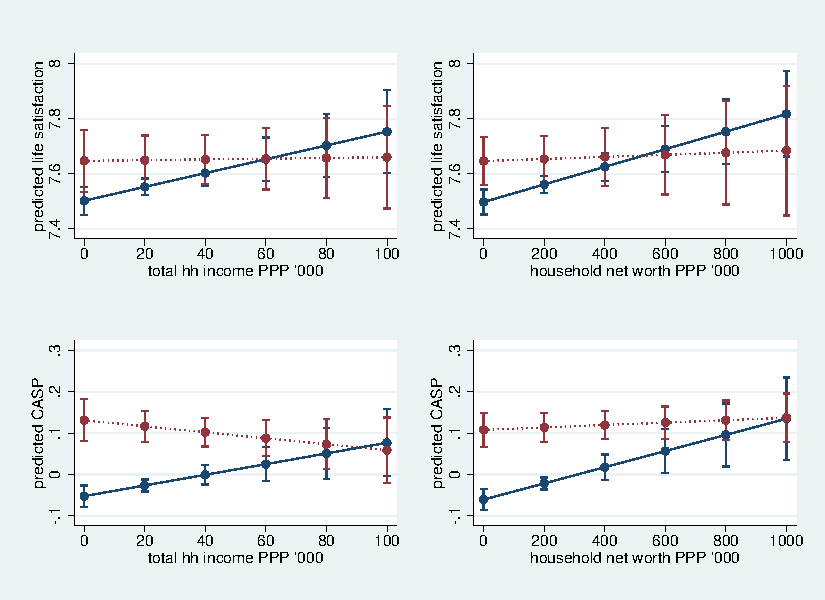
\includegraphics[width=4in]{/tmp/shareElderly/regDmarg.pdf}  
  \caption{dsfsadfsdaf}
  \label{mar}
\end{figure}


% or take scanario of middle class family with ??? v rich family ???: for the midlle
% class the rlationship betwene volnteering and swb is about 2x
%there are some such results in dofile


Neighborhood support groups have always played a key role in helping the poor
survive \citep{saegert2002social}, and so do individual persons play a key role
helping other poor \citep{mazelis2017surviving}. Most countries experience
rising inequality \citep{piketty03,mackintosh13,oecd08,verbeek15}--the middle
class is diminishing\footnote{For the world as a whole, the inequality is
  decreasing due to the poor countries, notably China, catching up--in many poor
  countries, middle class is actually increasing.}, and it is becoming two classes: the rich and the
rest. Volunteering may not be the viable strategy for the rich, but it is for the rest. 


Interestingly, additional results (see supplementary material) show that the
relationship with pension is opposite to that of total income--the higher the
pension, the stronger the effect from volunteering.\footnote{although results are
statistically insiginificant for life staistafction and only significant for CASP} One explanation is that
pensions do not require time (as opposed to labor income), and provide peace of
mind and let one engage in volunteering as opposed to paid labor. 
Likewise, additional results (see supplementary material) indicate that elders
who are retired derive more wellveing from volunteering. This makes sense--they
have more time and lower opportunity cost. 


\section{conclusion and discussion}

This study adds another piece of evidence to a line of research arguing that
volunteering is a productive aging strategy \citep[e.g.,][]{wilson12B,hank09}.
It is especially important given that the burden of aging %hank05 used the term
 is increasing--all European countries are aging--and younger generations will
 have to increasingly pay more for the elderly.

Volunteering (or anything else for that matter) cannot be a complete alternative
or a substitute to social transfers--one needs to be able to afford necessities.
But it can be a significant complement and
it can tradeoff some of the decrease in transfers.

These are very rich data and tehre can be much more done in terms of narrowing
doen and mersuring pensions and volunteering. The goal of this study was hovewer
to focus on the general relationship and the tadeoff between the two.

Futre research could look at earlier life experiences effect on successful
againg. For instance, in the US \citet{pruchno10} found that incarceration
 marital, work, and volunteer statuses, as well as moderate
alcohol consumption affect succesful again--such approach could be
replicated in Europe using SHARELIFE, SHARE module focused on people's life
histories. In particular, it would be interesting to examine effect of earlier
volunteering in life on succesful aging later in life--perhaps, not only
volunteering later in life, but also earlier has a positive effect. 


in this study we focused on overal patterns (controling for country level fixed
effects). furture research can explore differences across countries. 

As any correlational study, causality cannot be established

% %table centered on decimal points:)
% \begin{table}[H]\centering\footnotesize
% \caption{\label{freq_im_god} importance of God}
% \begin{tabular} {@{} lrrrr @{}}   \hline 
% Item& Number & Per cent   \\ \hline
% 1(not at all)&    9,285&  9\\
% 2&    3,555&        3\\
% 3&    3,937&        4\\
% 4&    2,888&        3\\
% 5&    7,519&        7\\
% 6&    5,175&        5\\
% 7&    6,050&        6\\
% 8&    8,067&        8\\
% 9&    8,463&        8\\
% 10&   52,385&       49\\
% Total&  107,324&      100\\ \hline
% \end{tabular}\end{table}


% % Define block styles
% \tikzstyle{block} = [rectangle, draw, fill=black!20, 
%     text width=10em, text centered, rounded corners, minimum height=4em]
% \tikzstyle{b} = [rectangle, draw,  
%     text width=6em, text centered, rounded corners, minimum height=4em]
% \tikzstyle{line} = [draw, -latex']
% \tikzstyle{cloud} = [draw, ellipse,fill=black!20, node distance = 5cm,
%     minimum height=2em]
    
% \begin{tikzpicture}[node distance = 2cm, auto]
%     % Place nodes
%     \node [block] (lib) {liberalism, egalitarianism, welfare};
%     \node [block, below of=lib] (con) {conservatism, competition, individualism};
%     \node [cloud, right of=con] (ls) {well-being};
%     \node [block, below of=ls] (cul) {genes, culture};
%     \node [b, left of =lib, node distance = 4cm] (c) {country-level};
%     \node [b, left of =con,  node distance = 4cm] (c) {person-level};
%     % Draw edges
%     \path [line] (lib) -- (ls);
%     \path [line] (con) -- (ls);
%     \path [line,dashed] (cul) -- (ls);
% \end{tikzpicture}


%PUT THIS NOTE, polish and put to /root/author_what_data --ALWAYS
%stick here stuff as i run it!!! maybe comment out later...


TODO: have separate som-r.tex as opposed to having it below; and in paper say
see supplemetary material as opposed to see appendix!

% \section*{\Huge ONLINE APPENDIX}
% \textbf{[note: this section will NOT be a part of the final version of
%   the manuscript, but will be available online instead]} %hence everything below
%                                 %is organized byu section, not subsection
% !!!
% have most of the stuff outputted to online appendix:)--start with that and then
% select stuff to paper--have brief narrative describng patterns in online app too
% !!!

% \section*{Variables' definitions, coding, and distributions}
% \label{app_var_des}


% %\input{/tmp/a.tex} %aok_var_des

% % \begin{spacing}{.9}
% %   \begin{table}[H]\centering \caption{Summary statistics.} \label{sumSta} \begin{scriptsize} \begin{tabular}{p{1.8in}p{.5in}p{.5in}p{.5in}p{.5in}p{.5in}p{.5in}p{.5in}p{.5in}p{.5in}p{.5
% %             in}p{.5in}p{.5 in}}\hline
% %         \input{/tmp/aha2.tex}
% %          \end{tabular}\end{scriptsize}\end{table}
% % \end{spacing}

% % \begin{spacing}{.9}
% %   \begin{table}[H]\centering \caption{Correlation matrix.} \label{sumSta} \begin{scriptsize} \begin{tabular}{@{}
% %           p{1.2in} rrrrrrrrrrrrr @{}}\hline
% %         \input{/tmp/ahb2.tex}\hline
% %          \end{tabular}\end{scriptsize}\end{table}
% % \end{spacing}



% Table XXX shows variable distributions. If a variable has more than
% 10 categories it is classified into bins...

% %\input .... %TODO !!!! have input here histograms

% \section*{Additional Descriptive Statistics}
% \label{app_des_sta}

% %make sure i have [H] or h! ???
% % \begin{table}[H]
% % \caption{}
% % \centering
% % \label{}
% % \begin{scriptsize}
% % \input{../out/reg_c.tex}
% % \end{scriptsize}
% % \end{table}

%\newpage
%\theendnotes
\bibliography{/home/aok/papers/root/tex/ebib.bib,socTraSocCap.bib}

{\huge Supplementary Online Material}

\section{appendix: additional descriptive statistics}

\begin{table}[H]\centering\footnotesize
 \caption{\label{var_des} Variable definitions.}
\begin{tabular} {p{1.5in}p{4.5in}}   \hline
name & description   \\ \hline
  swb & "On a scale from 0 to 10 where 0 means completely dissatisfied and 10 means completely satisfied, how satisfied are you with your life?" [imputed] \\
  casp & casp scale: see table \\ref{casp} [ac] \\
\hline\end{tabular}\end{table} 
{\footnotesize [imputed], [ac], and [sp] pertain to SHARE modules.}
\begin{table}[H]\centering\footnotesize
 \caption{\label{var_des} Variable definitions.}
\begin{tabular} {p{1.5in}p{4.5in}}   \hline
name & description   \\ \hline
  voluntary or charity work & "Please look at card 38: which of the activities listed on this card - if any - have you done in the past twelve months?" "Done voluntary or charity work" [ac] \\
  how often done voluntary or charity work & "How often in the past twelve months did you [do voluntary or charity work/cared for a sick or disabled adult/provided help to friends or neighbors/attended an educational or training course/go to a sport, social or other kind of club/taken part in the activities of a religious organization (church, synagogue, mosque etc.)/taken part in a political or community-related organization/read books, magazines or newspapers/do word or number games such as crossword puzzles or Sudoku/play cards or games such as chess]?" [ac] \\
  attended an educational or training course & "Please look at card 38: which of the activities listed on this card - if any - have you done in the past twelve months?" "Done voluntary or charity work" [ac]  [ac] \\
  gone to a sport, social or other kind of club & "Please look at card 38: which of the activities listed on this card - if any - have you done in the past twelve months?" "Done voluntary or charity work" [ac]  [ac] \\
  taken part in a political or community-related organization & "Please look at card 38: which of the activities listed on this card - if any - have you done in the past twelve months?" "Done voluntary or charity work" [ac]  [ac] \\
  read books, magazines or newspapers & "Please look at card 38: which of the activities listed on this card - if any - have you done in the past twelve months?" "Done voluntary or charity work" [ac]  [ac] \\
  did word or number games (crossword puzzles/Sudoku...) & "Please look at card 38: which of the activities listed on this card - if any - have you done in the past twelve months?" "Done voluntary or charity work" [ac]  [ac] \\
  played cards or games such as chess & "Please look at card 38: which of the activities listed on this card - if any - have you done in the past twelve months?" "Done voluntary or charity work" [ac]  [ac] \\
\hline\end{tabular}\end{table} 
{\footnotesize [imputed], [ac], and [sp] pertain to SHARE modules.}
\begin{table}[H]\centering\footnotesize
 \caption{\label{var_des} Variable definitions.}
\begin{tabular} {p{1.5in}p{4.5in}}   \hline
name & description   \\ \hline
  annual old age, early retirement pensions, survivor and war pension & EP078\_1-2-3-7-8-9 (1-2-3-9-10-11 in w6)  "After taxes, about how large was a typical payment of [ your public old age pension/ your public old age supplementary pension or public old age second pension/ your public early retirement or pre-retirement pension/ your main public sickness benefits/ your main public disability insurance pension/ your secondary public disability insurance pension/ your Secondary public sickness benefits/ your public unemployment benefit or insurance/ your main public survivor pension from your spouse or partner/ your secondary public survivor pension from your spouse or partner/ your public war pension/ your public long-term care insurance/ your social assistance] in [STR (Year - 1)]?" [imputed] \\
  annual private occupational pensions & "After taxes, what was the approximate annual amount received from all your occupational pensions in [STR (Year - 1)]?" [imputed] \\
  other regular payments from private pernsions & "After any taxes and contributions, about how large was the average payment of [ you life insurance payments from a private insurance company/ your private annuity or private personal pension payments/ your alimony/ your regular payments from charities/ your long-term care insurance payments] in [STR (Year - 1)]?" [imputed] \\
  pension & EP078\_1-2-3-7-8-9 (1-2-3-9-10-11 in w6) from annual old age, early retirement pensions, survivor and war pension AND from annual private occupational pensions AND other regular payments from private pernsions  [imputed] \\
  disability/sickness benefits & EP078\_5-6  and EP078\_3\_6\_10 (4-7 in w6) [from question in "annual old age, early retirement pensions, survivor and war pension"] [imputed] \\
  unemployment benefits & EP078\_6 (8 in w6) [from question in "annual old age, early retirement pensions, survivor and war pension"] [imputed] \\
  social assistance & EP078\_10 (12-13 in w6) [from question in "annual old age, early retirement pensions, survivor and war pension"] [imputed] \\
\hline\end{tabular}\end{table} 
{\footnotesize [imputed], [ac], and [sp] pertain to SHARE modules.}
\begin{table}[H]\centering\footnotesize
 \caption{\label{var_des} Variable definitions.}
\begin{tabular} {p{1.5in}p{4.5in}}   \hline
name & description   \\ \hline
  labor income & "After any taxes and contributions, what was your approximate annual income from employment in the year [STR (Year - 1)]? Please include any additional or extra or lump sum payment, such as bonuses, 13 month, Christmas or Summer pays." AND "After any taxes and contributions and after paying for any materials, equipment or goods that you use in your work, what was your approximate annual income from self-employment in the year [STR (Year - 1)]?" [imputed] \\
  household net worth & calculated variable--see Release Guide 6.0.0 [imputed] \\
  years of education & "How many years have you been in full-time education?" full-time education * includes: receiving tuition, engaging in practical work or supervised study or taking examinations * excludes: full-time working, home schooling, distance learning, special on-the-job training, evening classes, part-time private vocational training, flexible or part-time higher education studies, etc  [imputed] \\
  age & Age of respondent (based on interview year)  "In which month and @byear@b were you born?" [imputed] \\
  male & OBSERVATION Note sex of respondent from observation (ask if unsure) \\
  self reported health & "Would you say your health is..." "Poor"..."Excellent" [imputed] \\
  married and living together & "What is your marital status?"  [imputed] \\
  employed & The following questions are about your current main job. "In this job were you a private-sector employee, a public sector employee or self-employed?"  [imputed] \\
  number of children & "Now I will ask some questions about your children. How many children do you have that are still alive? Please count all natural children, fostered, adopted and stepchildren [ , including those of/ , including those of/ , including those of/ , including those of] [ your husband/ your wife/ your partner/ your partner] [ {Name of partner/spouse}]." [imputed] \\
\hline\end{tabular}\end{table} 
{\footnotesize [imputed], [ac], and [sp] pertain to SHARE modules.}

PEr historgams note: Because we mostly use imputed dataset some values are not integers even when base
question does not include fraction such as dummy variable for being married. 


 \begin{figure}[H] \centering 
\subfloat{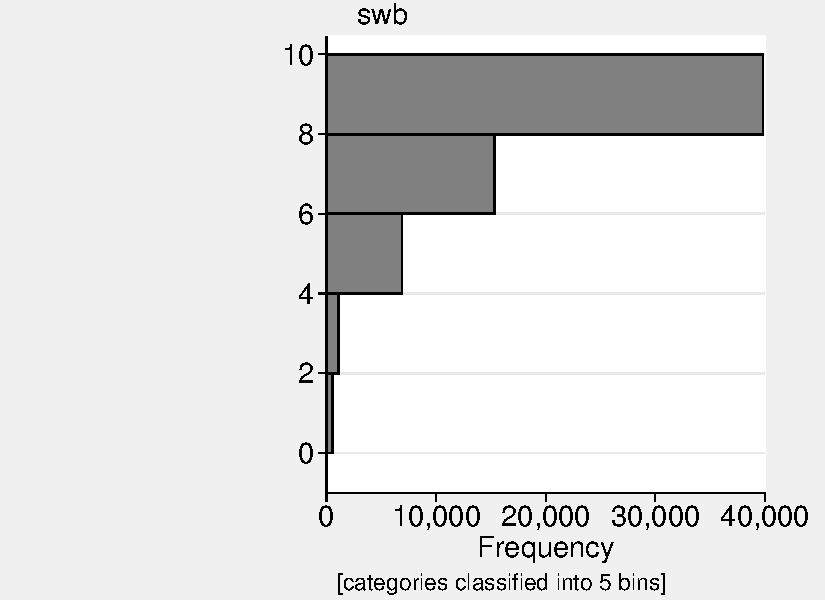
\includegraphics[width=1.7in]{hist-11.pdf}}
\subfloat{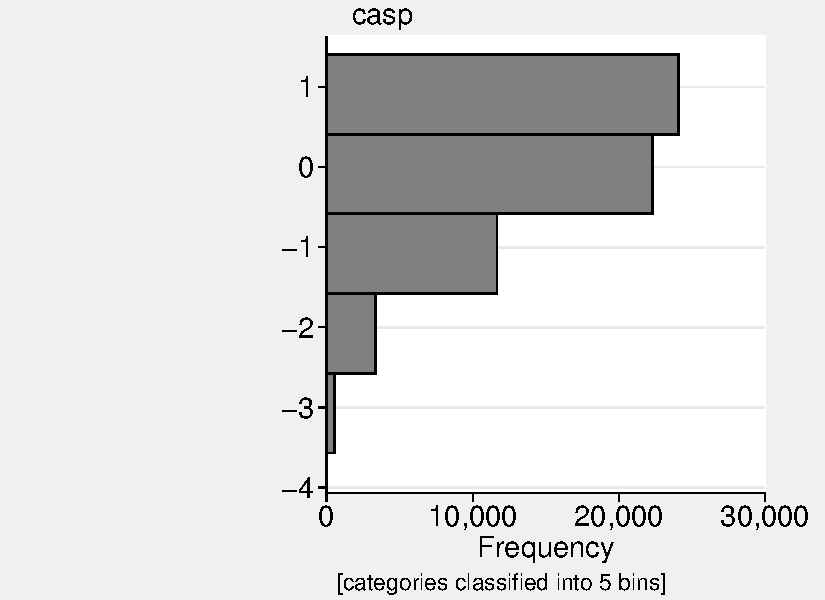
\includegraphics[width=1.7in]{hist-12.pdf}}
  \vspace{.15in} \caption{Variables' distribution.} \label{hist} \end{figure} 

 \begin{figure}[H] \centering 
\subfloat{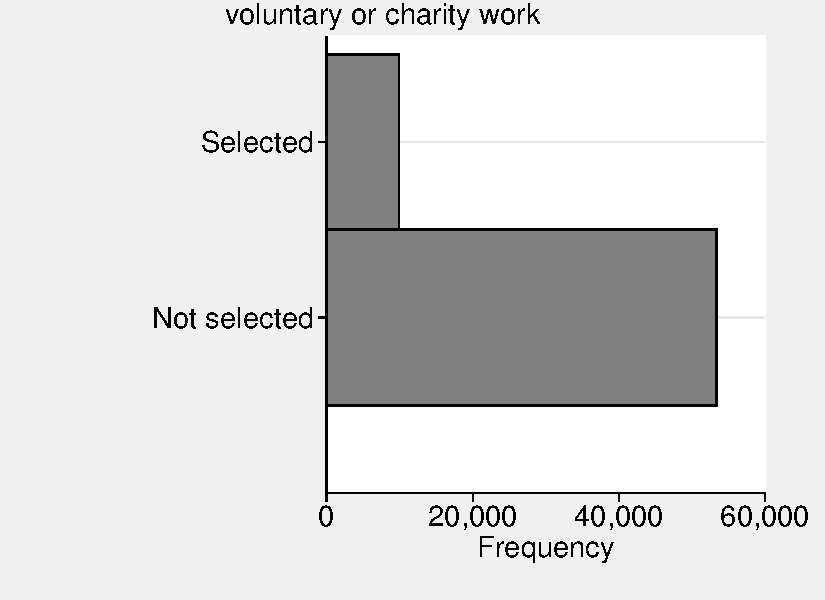
\includegraphics[width=1.7in]{hist-21.pdf}}
\subfloat{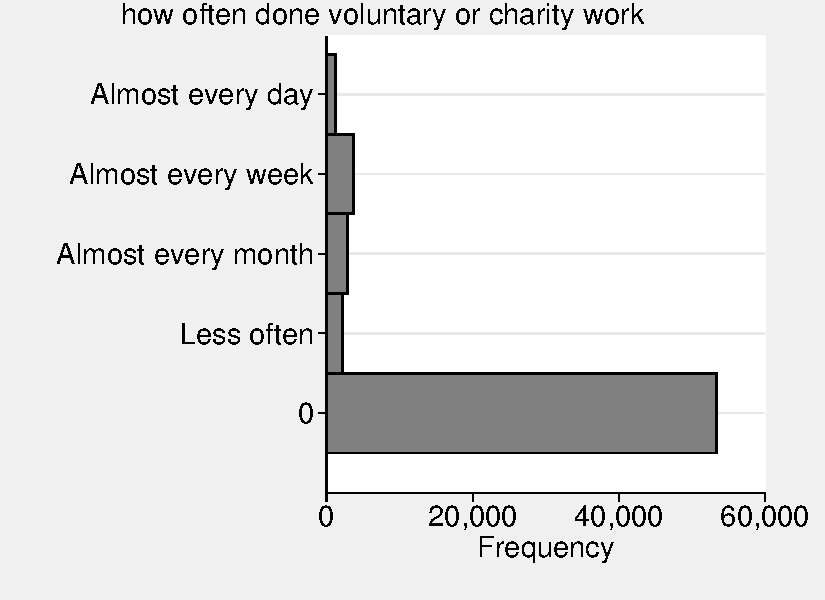
\includegraphics[width=1.7in]{hist-22.pdf}}
\subfloat{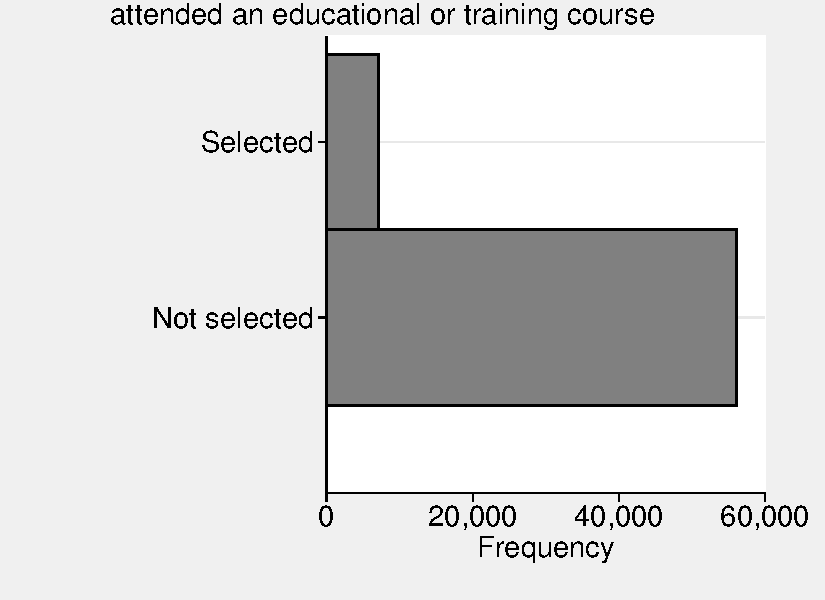
\includegraphics[width=1.7in]{hist-23.pdf}}\\ \vspace{-.15in}
\subfloat{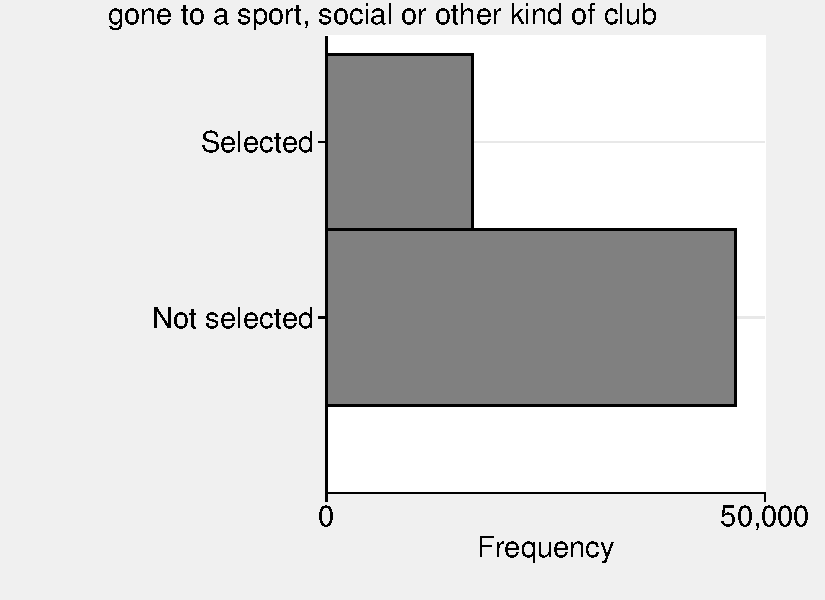
\includegraphics[width=1.7in]{hist-24.pdf}}
\subfloat{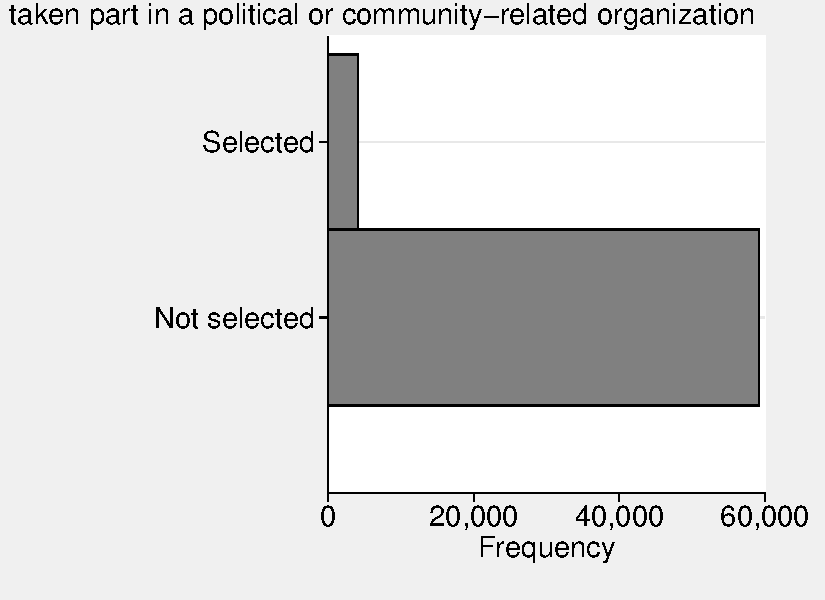
\includegraphics[width=1.7in]{hist-25.pdf}}
\subfloat{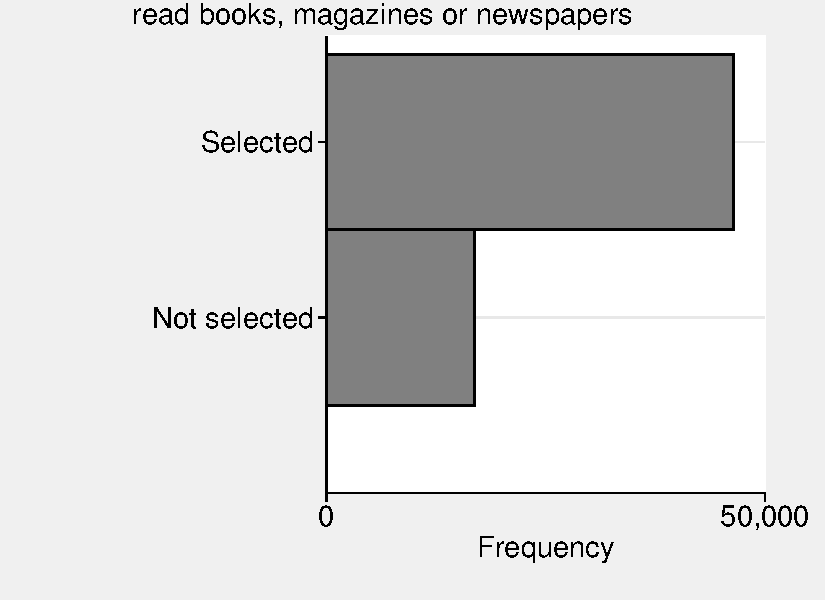
\includegraphics[width=1.7in]{hist-26.pdf}}\\ \vspace{-.15in}
\subfloat{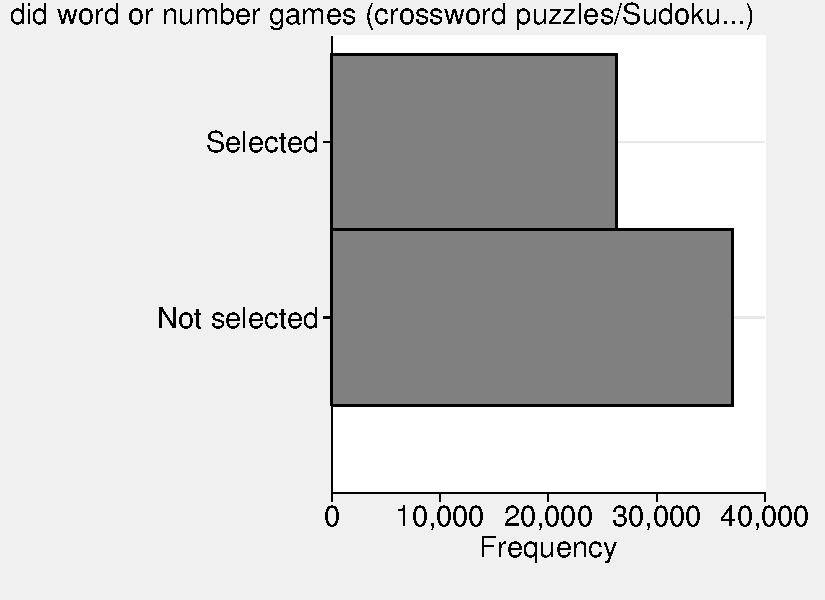
\includegraphics[width=1.7in]{hist-27.pdf}}
\subfloat{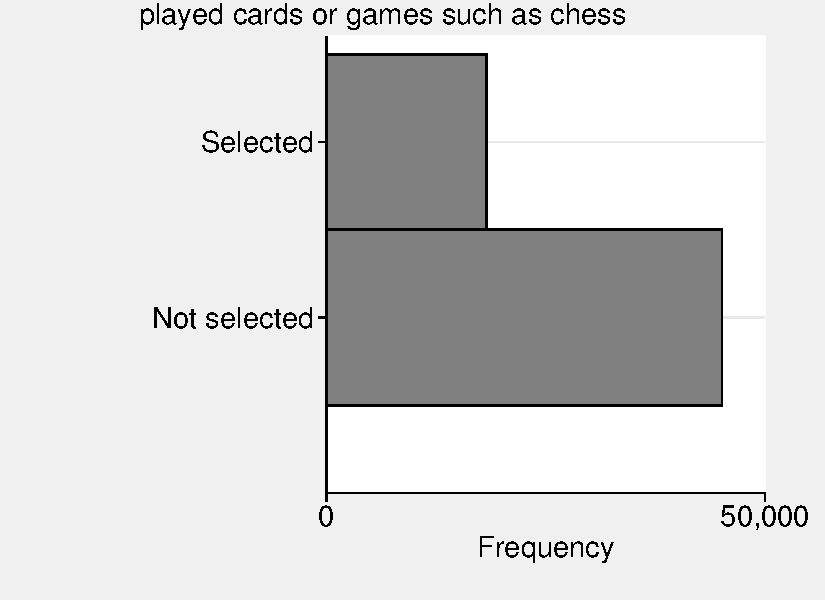
\includegraphics[width=1.7in]{hist-28.pdf}}
  \vspace{.15in} \caption{Variables' distribution.} \label{hist} \end{figure} 

 \begin{figure}[H] \centering 
\subfloat{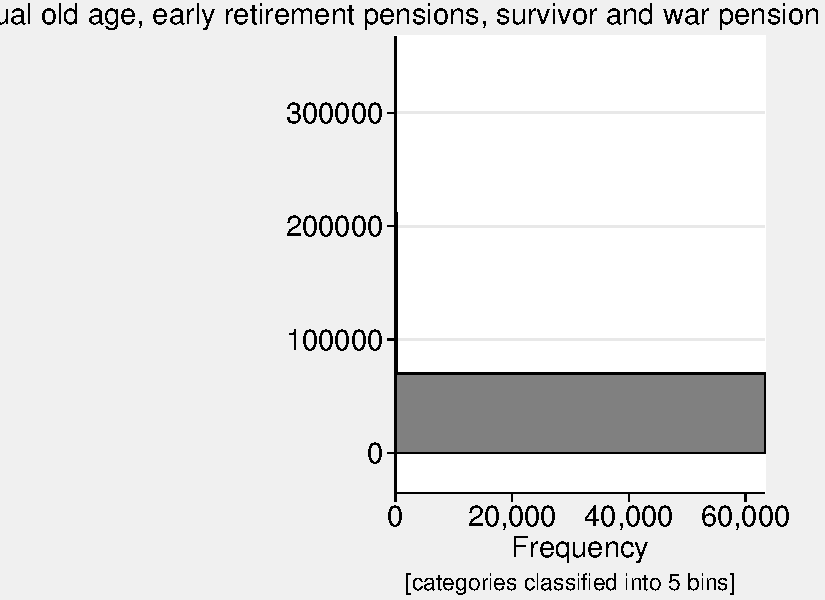
\includegraphics[width=1.7in]{hist-31.pdf}}
\subfloat{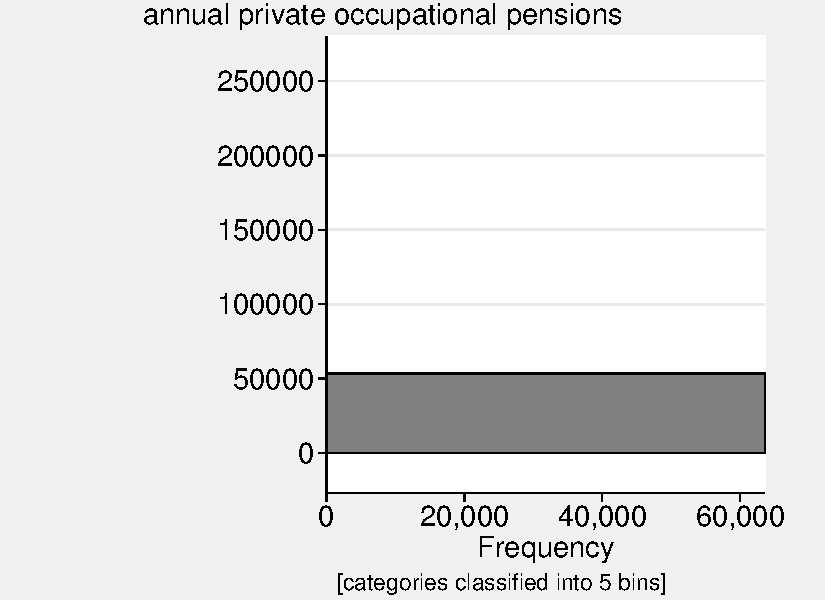
\includegraphics[width=1.7in]{hist-32.pdf}}
\subfloat{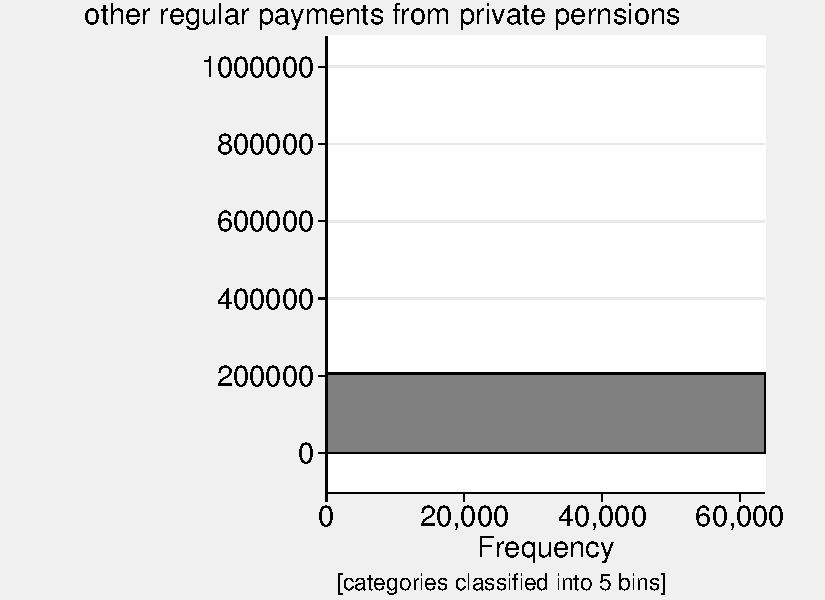
\includegraphics[width=1.7in]{hist-33.pdf}}\\ \vspace{-.15in}
\subfloat{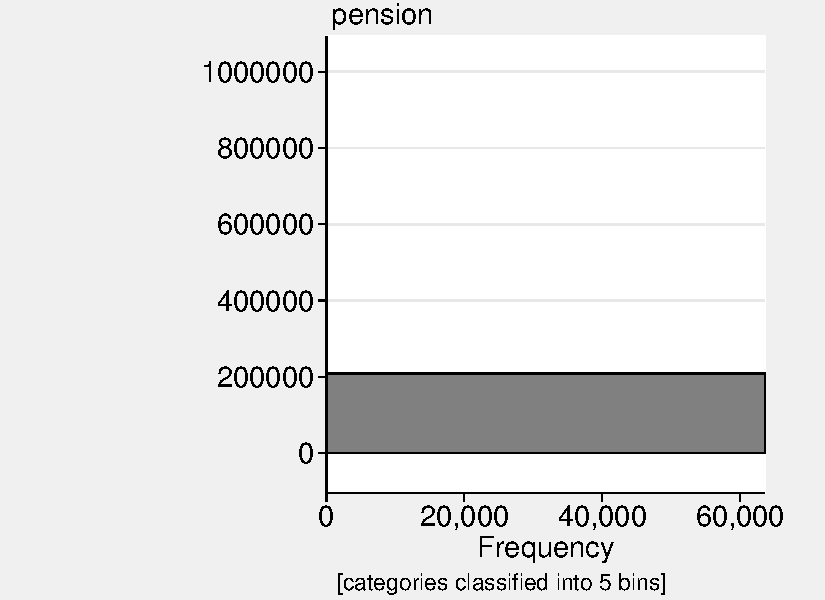
\includegraphics[width=1.7in]{hist-34.pdf}}
\subfloat{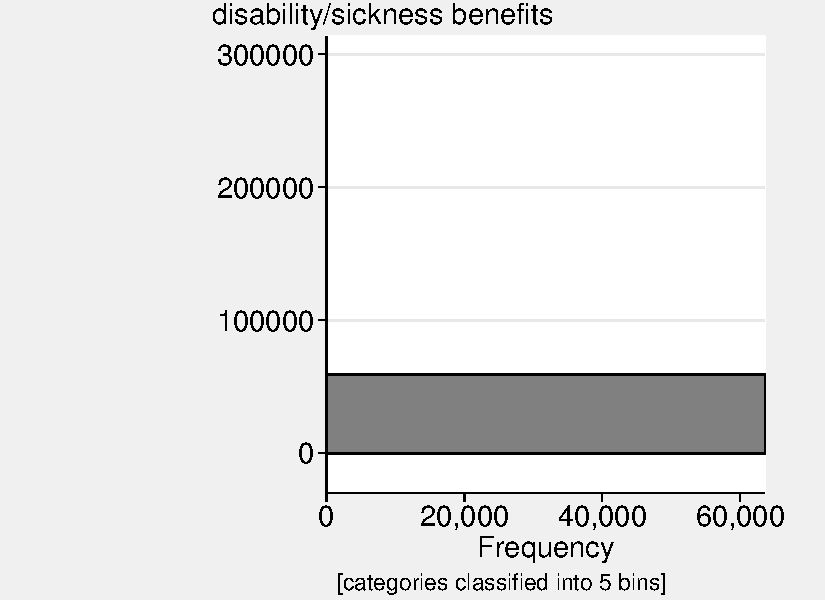
\includegraphics[width=1.7in]{hist-35.pdf}}
\subfloat{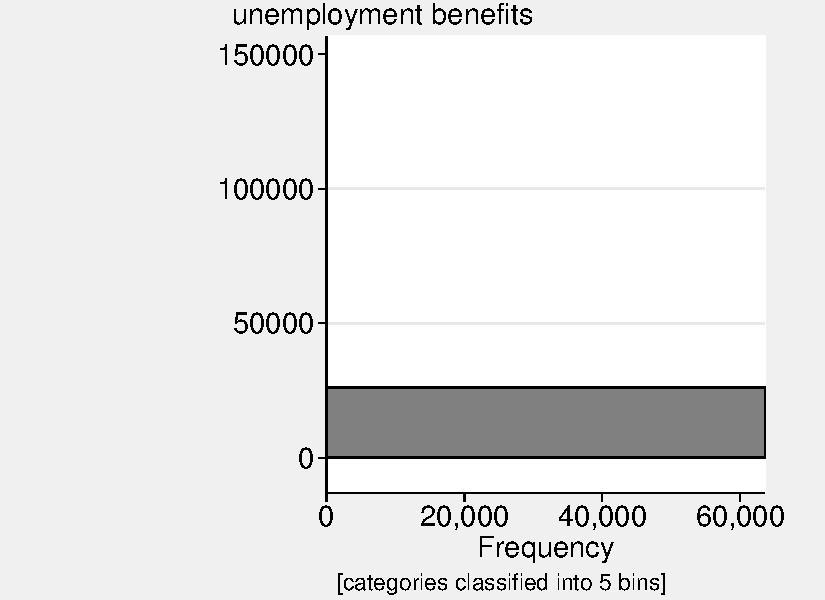
\includegraphics[width=1.7in]{hist-36.pdf}}\\ \vspace{-.15in}
\subfloat{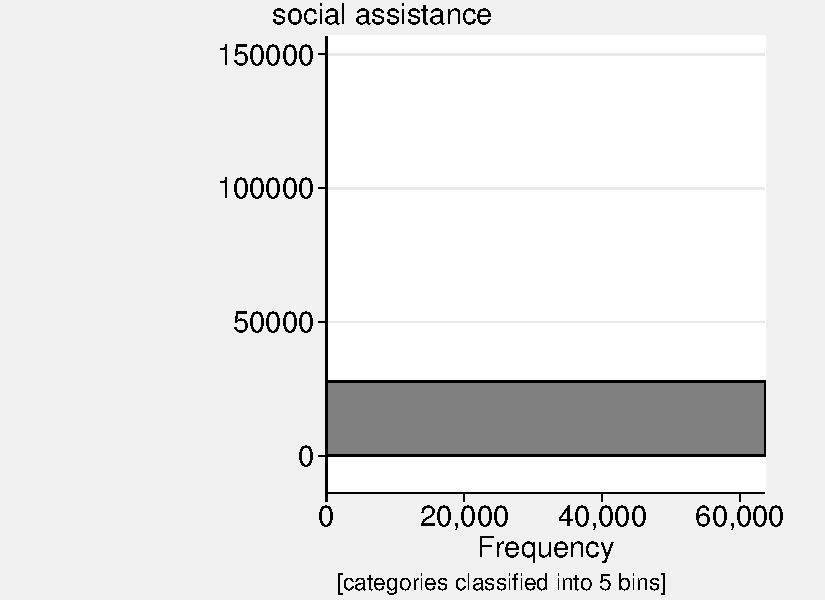
\includegraphics[width=1.7in]{hist-37.pdf}}
  \vspace{.15in} \caption{Variables' distribution.} \label{hist} \end{figure} 

 \begin{figure}[H] \centering 
\subfloat{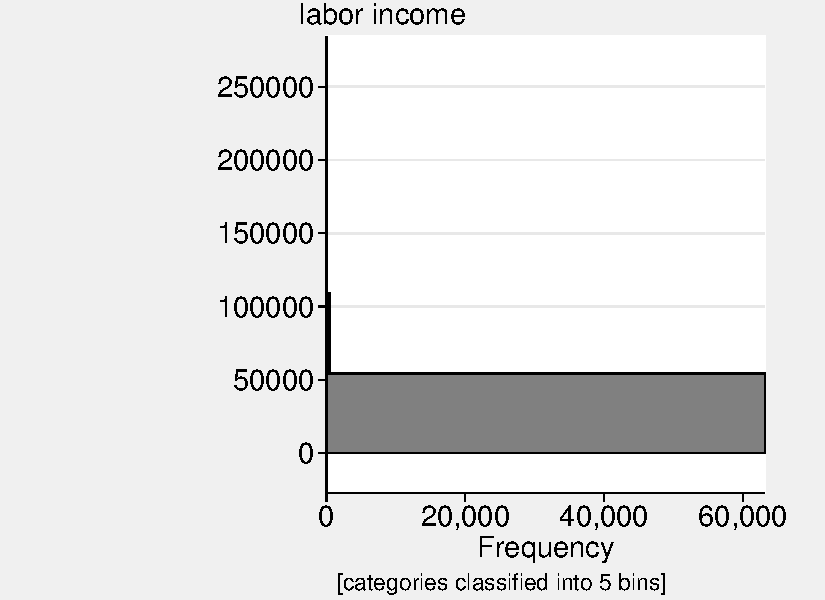
\includegraphics[width=1.7in]{/tmp/shareElderly/hist-41.pdf}}
\subfloat{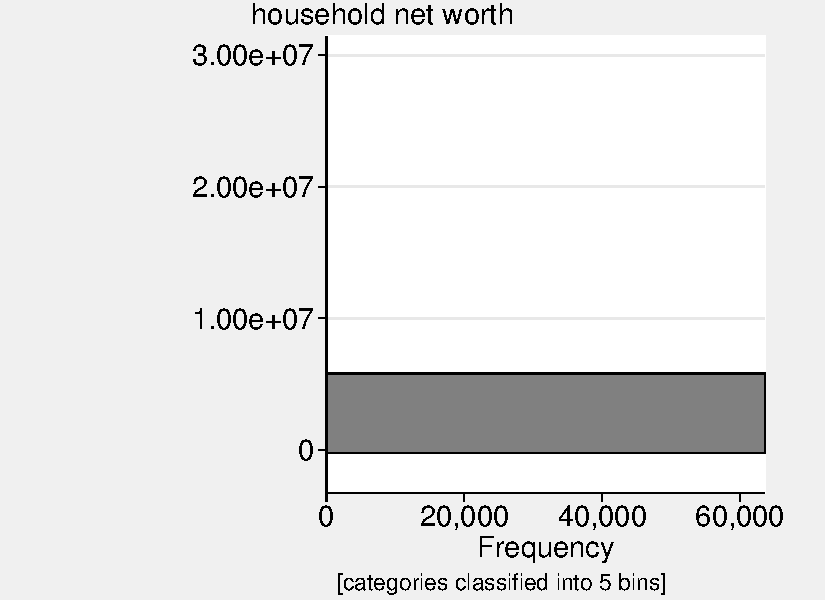
\includegraphics[width=1.7in]{/tmp/shareElderly/hist-42.pdf}}
\subfloat{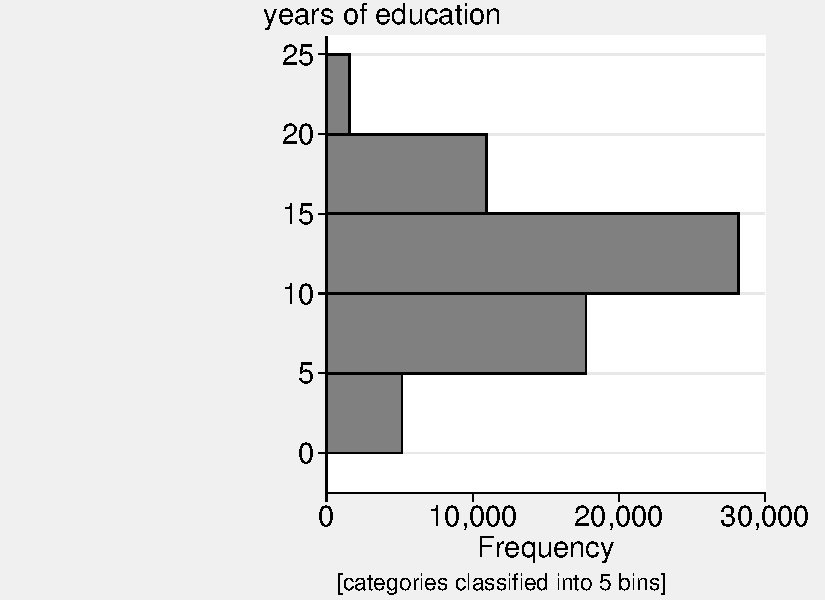
\includegraphics[width=1.7in]{/tmp/shareElderly/hist-43.pdf}}\\ \vspace{-.15in}
\subfloat{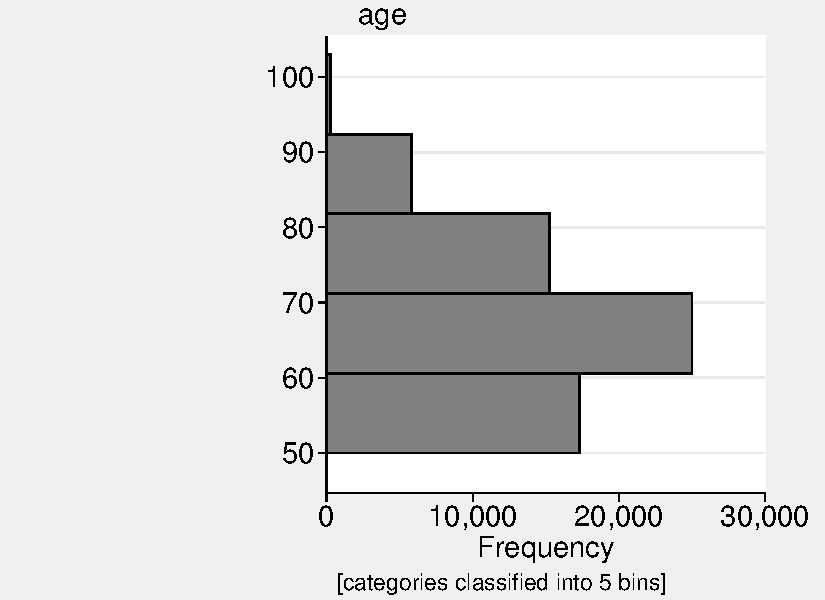
\includegraphics[width=1.7in]{/tmp/shareElderly/hist-44.pdf}}
\subfloat{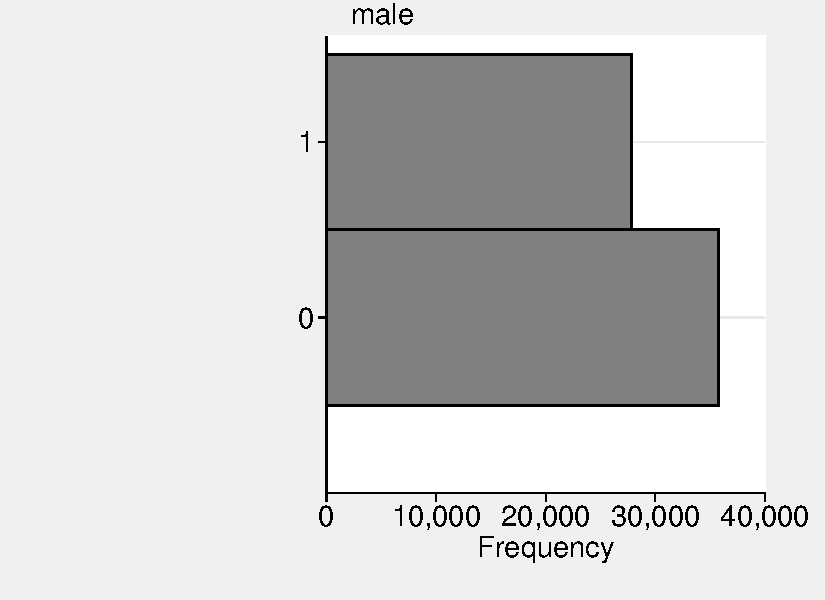
\includegraphics[width=1.7in]{/tmp/shareElderly/hist-45.pdf}}
\subfloat{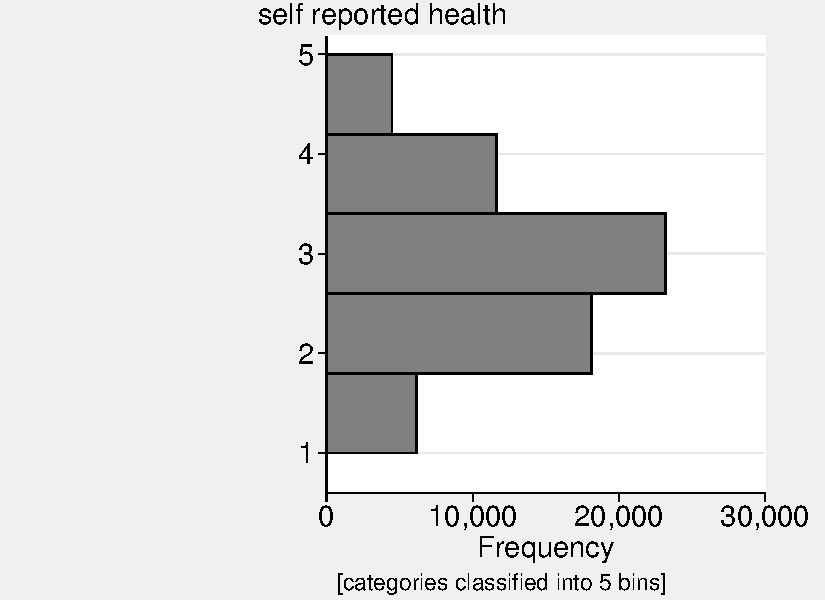
\includegraphics[width=1.7in]{/tmp/shareElderly/hist-46.pdf}}\\ \vspace{-.15in}
\subfloat{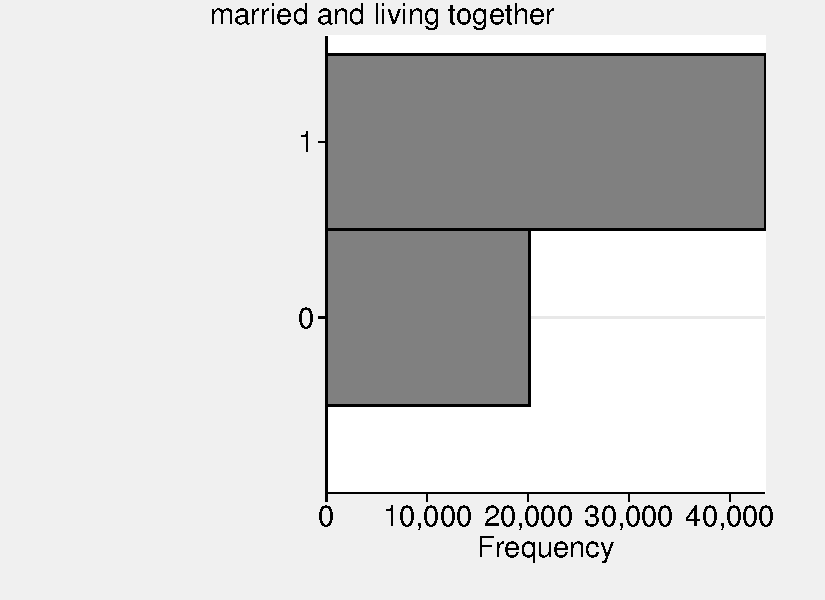
\includegraphics[width=1.7in]{/tmp/shareElderly/hist-47.pdf}}
\subfloat{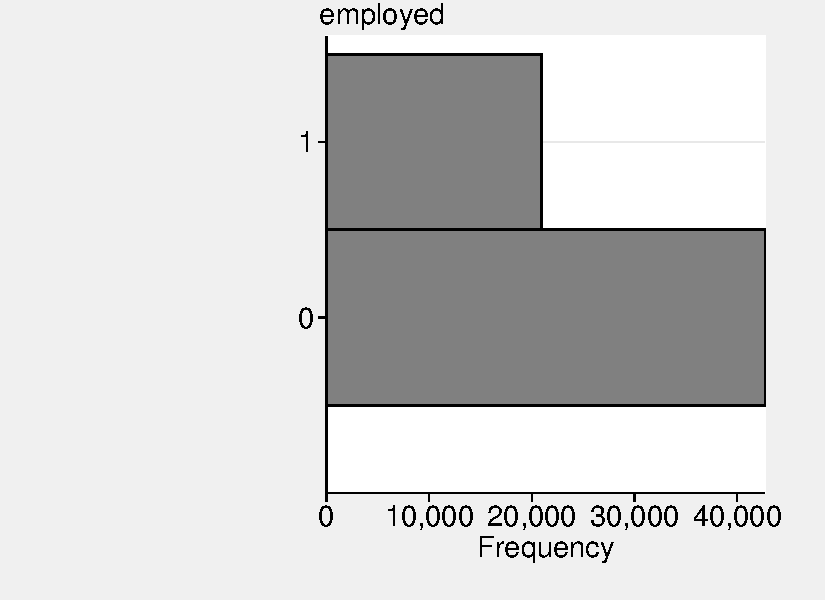
\includegraphics[width=1.7in]{/tmp/shareElderly/hist-48.pdf}}
\subfloat{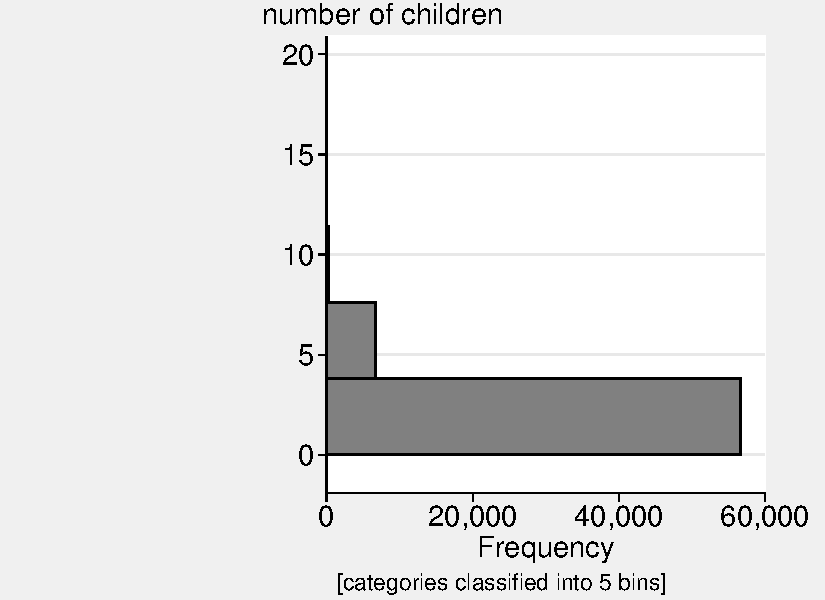
\includegraphics[width=1.7in]{/tmp/shareElderly/hist-49.pdf}}\\ \vspace{-.15in}
  \vspace{.15in} \caption{Variables' distribution.} \label{hist} \end{figure} 



\begin{spacing}{.9}
\begin{table}[H]\centering \caption{OLS of SWB  (life satisfaction and CASP) on
    volunteerring and pensions.  Unstandarized coefficients reported.}  \begin{scriptsize} \begin{tabular}{p{1.8in}p{.5in}p{.5in}p{.5in}p{.5in}|p{.5in}p{.5in}p{.5in}p{.5in}p{.5in}p{.4in}p{.5in}p{.4in}}\hline &\multicolumn{4}{c}{Life satisfaction}&\multicolumn{4}{c}{CASP}\\
                    &          e1   &          e2   &          e3   &          e4   &          e5   &          e6   &          e7   &          e8   \\
no voluneering/charity&      0.0000   &      0.0000   &      0.0000   &      0.0000   &      0.0000   &      0.0000   &      0.0000   &      0.0000   \\
voluneering/charity &      0.4611***&      0.1433** &      0.3380***&      0.0629   &      0.4497***&      0.1860***&      0.3544***&      0.1140***\\
employed=0          &      0.0000   &      0.0000   &               &               &               &               &               &               \\
employed=1          &      0.2869***&      0.1681***&               &               &               &               &               &               \\
no voluneering/charity $\times$ employed=0&      0.0000   &      0.0000   &               &               &               &               &               &               \\
no voluneering/charity $\times$ employed=1&      0.0000   &      0.0000   &               &               &               &               &               &               \\
voluneering/charity $\times$ employed=0&      0.0000   &      0.0000   &               &               &               &               &               &               \\
voluneering/charity $\times$ employed=1&     -0.2571** &     -0.1472+  &               &               &               &               &               &               \\
employed            &               &               &               &      0.1460** &      0.4270***&      0.0000   &               &      0.0894***\\
total hh income PPP '000&               &      0.0023** &               &      0.0028***&               &               &               &      0.0009*  \\
Total household expenditure PPP '000&               &      0.0030   &               &      0.0021   &               &      0.0078***&               &      0.0066***\\
household net worth PPP '000&               &      0.0003***&               &               &               &      0.0002***&               &               \\
attended an educational or training course&               &      0.0432   &               &      0.0446   &               &      0.0567** &               &      0.0548** \\
gone to a sport, social or other kind of club&               &      0.1619***&               &      0.1711***&               &      0.1284***&               &      0.1326***\\
taken part in a political or community-related organization&               &     -0.0081   &               &     -0.0050   &               &      0.0534*  &               &      0.0535*  \\
read books, magazines or newspapers&               &      0.2992***&               &      0.3075***&               &      0.2162***&               &      0.2201***\\
did word or number games (crossword puzzles/Sudoku...)&               &      0.0664*  &               &      0.0649+  &               &      0.0787***&               &      0.0769***\\
played cards or games such as chess&               &      0.1018** &               &      0.1013** &               &      0.0585***&               &      0.0576***\\
male                &               &      0.0289   &               &      0.0286   &               &      0.0783***&               &      0.0732***\\
married and living together&               &      0.5362***&               &      0.5511***&               &      0.1677***&               &      0.1744***\\
age                 &               &      0.0265***&               &      0.0269***&               &      0.0003   &               &      0.0000   \\
years of education  &               &      0.0020   &               &      0.0038   &               &      0.0073***&               &      0.0079***\\
number of children  &               &      0.0122   &               &      0.0115   &               &     -0.0088   &               &     -0.0090   \\
self reported health&               &      0.5470***&               &      0.5528***&               &      0.3595***&               &      0.3625***\\
pension             &               &               &      0.0000** &     -0.0000   &               &               &      0.0000   &      0.0000   \\
no voluneering/charity $\times$ pension&               &               &      0.0000   &      0.0000   &               &               &      0.0000   &      0.0000   \\
voluneering/charity $\times$ pension&               &               &      0.0000   &      0.0000   &               &               &      0.0000   &      0.0000+  \\
no voluneering/charity $\times$ employed&               &               &               &               &      0.0000   &      0.0000   &               &               \\
voluneering/charity $\times$ employed&               &               &               &               &     -0.2543***&     -0.1320***&               &               \\
country dummies&yes&yes&yes&yes&yes&yes&yes&yes\\
constant            &      8.0711***&      3.8225***&      8.1191***&      3.8005***&      0.1479***&     -1.4125***&      0.2886***&     -1.3963***\\
N                   &       62967   &       62967   &       62967   &       62967   &       61492   &       61492   &       61492   &       61492   \\

      \hline\multicolumn{5}{l}{+p$<$0.10 *p$<$0.05 **p$<$0.01 ***p$<$0.001,
        robust std err} \end{tabular}\label{regEw6w4} \end{scriptsize}\end{table}
\end{spacing}



\section{appendix: explanation of volunteering questions by SHARE expert}%from
                                %lm email by m oczkowska

In SHARE, there are also instructions for the pollster that appear on the
computer along with the question. For questions about volunteering (AC002 in w1
and w2 and AC035 in w4, w5, w6, w7) see column ``I'' ``iwer\_instruction'' in the
attached file (that is the same table you got as an expert).
For both questions the instructions are scanty: ``CODE ALL THAT APPLY.'' Only in
round 2 and round 4 is still the explanation of ``TAKING PART IN THE ACTIVITIES
OF A RELIGIOUS ORGANIZATION INCLUDES CHURCH ATTENDANCE.'' Because in these
rounds in the answers option was ``taking part in activities of a religious
organization.'' There is nothing about what we mean by
volunteering. Interviewers are trained to write what the respondent says and do
not ask. In exceptional situations, as the respondent asks what the term means,
they may explain, but I have never heard anyone ask what volunteering is. Plus
if they have doubts whether the respondent is actually what they ask, they can
write a note (what they do often, but just for volunteering I do not remember to
write something before).

On the other hand, my personal opinion is this: the question of activity in this
volunteering is at the end of the survey. Ask for help for family members or
other people, ask for financial gifts / gifts and take care of your
grandchildren beforehand. I think if someone helps in these categories it takes
into account this before and not as volunteering.
In addition, the question of volunteering is quite concrete and formal ``Done
voluntary or charity work'', which in Polish version is ``Participation in
charitable activities or volunteering''. I doubt anyone would understand this as
helping grandpa. I think the wording is good and captures only the involvement
in external ``volunteering''. But of course it will also depend on the language
version.
Let me know if I helped,

\end{spacing}
\end{document}
